\documentclass{book}

\usepackage[T1,T2A]{fontenc}
\usepackage[utf8]{inputenc}
\usepackage[ukrainian]{babel}
\usepackage{makeidx}
\usepackage[unicode]{hyperref}
\usepackage[symbol]{footmisc}
\usepackage{marvosym}
\usepackage{amsmath}
\usepackage{amssymb}
\usepackage{graphicx}
\usepackage{caption}
\usepackage{subcaption}
\usepackage{environ}
\usepackage{tikz}
\usepackage{enumitem}
\usepackage{longtable}
\usepackage{afterpage}
\usepackage{verbatimbox}
\usepackage{pmboxdraw}
\usepackage{calc}
\usepackage{menukeys}
\usepackage{graphicx}
\usepackage{xifthen}

\DeclareRobustCommand{\hryvnia}{{%
  \fontencoding{OT1}\upshape
  \settoheight{\dimen255}{S}%
  \vphantom{S}%
  \smash{\ooalign{%
    \hfil\reflectbox{S}\hfil\cr % a reflected S
    \hfil\raisebox{0.10ex}{-}\hfil\cr % upper bar
    \hfil\raisebox{-0.11ex}{-}\hfil\cr % lower bar
  }}%
}}

\DeclareUnicodeCharacter{20B4}{\hryvnia}
\DeclareTextSymbolDefault{\dh}{T1}
\DeclareMathOperator{\abs}{\hbox{\texttt{abs}}}

\pmboxdrawsetup{
  Block/box={\texttt{0}},
  Shade/box={\texttt{0}},
}

\title{Робимо програми: шлях хакера}
\author{А. Мустіц}
\date{\today}
\makeindex

\renewcommand{\thefootnote}{\fnsymbol{footnote}}
\NewEnviron{exercise}{\par\goodbreak\smallskip\textbf{Вправа:} \BODY \par\smallskip}
\NewEnviron{summary}{\par\goodbreak\smallskip\textbf{Підсумки:}\begin{itemize} \BODY \end{itemize}\par\smallskip}

\NewEnviron{algorithm}{\medskip\goodbreak \BODY \medskip\goodbreak}
%\NewEnviron{algsteps}{\begin{enumerate}[\hspace{2\parindent}1.] \BODY \end{enumerate}}
\NewEnviron{algsteps}{\begin{enumerate}[
  topsep=0pt,itemsep=-1ex,partopsep=1ex,parsep=1ex,
  leftmargin=3\parindent
  ] \BODY \end{enumerate}}
\newcommand{\algcaption}[1]{\textbf{Алгоритм:} #1.\par}
\newcommand{\alginput}[1]{\textbf{Дано:} #1\par}
\newcommand{\algoutput}[1]{\textbf{Треба:} #1\par}
\newcommand{\algstep}{\item}
\newcommand{\algsummary}[1]{\par\textbf{Результат:} #1\par}

\newcommand{\bitstr}[1]{{\tt #1}}
\newcommand{\bitdesc}{послідовність бітів ми будемо писати моноширинним шрифтом, наприклад запис \bitstr{10011} означатиме послідовність п'яти біт \bitstr{1}, \bitstr{0}, \bitstr{0}, \bitstr{1} та \bitstr{1}.}

\newcommand{\hexstr}[1]{{\tt 0x#1}}
\newcommand{\hexdesc}{ми будемо записувати $16$--річні числа моноширинним шрифтом за префіксом {\tt 0x}, наприклад \hexstr{5A}}

\newcommand{\tritzero}{$\square$}
\newcommand{\trithalf}{\Yinyang}
\newcommand{\tritone}{$\blacksquare$}

\newcommand{\escape}[1]{\texttt{\char"5C #1}}
\newcommand{\textseq}[1]{\par\vbox{\texttt{~~~}#1}}
\newcommand{\id}[1]{\texttt{#1}}
\newcommand{\chr}[1]{«\texttt{#1}»}
\newcommand{\s}{\char"20}
\newcommand{\chspace}{\chr\s}
\newcommand{\chesc}[1]{\chr{\escape{#1}}}

\newcommand{\setunref}{\href{https://uk.wikipedia.org/wiki/\%D0\%A1\%D0\%B5\%D1\%82\%D1\%83\%D0\%BD\%D1\%8C_(\%D0\%BA\%D0\%BE\%D0\%BC\%D0\%BF\%27\%D1\%8E\%D1\%82\%D0\%B5\%D1\%80)}{https://uk.wikipedia.org/wiki/Сетунь\_(комп'ютер)}}
\newcommand{\quantumref}{\href{https://uk.wikipedia.org/wiki/\%D0\%9A\%D0\%B2\%D0\%B0\%D0\%BD\%D1\%82\%D0\%BE\%D0\%B2\%D0\%B8\%D0\%B9_\%D0\%BA\%D0\%BE\%D0\%BC\%D0\%BF\%27\%D1\%8E\%D1\%82\%D0\%B5\%D1\%80}{https://uk.wikipedia.org/wiki/Квантовий\_комп'ютер}}
\newcommand{\kruskalref}{\href{https://en.wikipedia.org/wiki/Kruskal\%27s_tree_theorem}{https://en.wikipedia.org/wiki/Kruskal\%27s\_tree\_theorem}}
\newcommand{\Gurtyak}{\href{https://uk.wikipedia.org/wiki/\%D0\%93\%D1\%83\%D1\%80\%D1\%82\%D1\%8F\%D0\%BA_\%D0\%94\%D0\%BC\%D0\%B8\%D1\%82\%D1\%80\%D0\%BE_\%D0\%9E\%D0\%BB\%D0\%B5\%D0\%BA\%D1\%81\%D0\%B0\%D0\%BD\%D0\%B4\%D1\%80\%D0\%BE\%D0\%B2\%D0\%B8\%D1\%87}{https://uk.wikipedia.org/wiki/Гуртяк\_Дмитро\_Олександрович}}

\newcommand{\unicode}[1]{«\bitstr{U+#1}»}
\newcommand{\encoding}[1]{%
    \ifthenelse{\equal{#1}{utf8}}{utf--8}{%
    \ifthenelse{\equal{#1}{utf16le}}{utf--16le}{%
    \ifthenelse{\equal{#1}{utf16be}}{utf--16be}{%
        ???}}}}

\begin{document}

\maketitle
\chapter{Світ, створений з біт}

Є мем: «справжні програмісти кодують програми у бінарному режимі».
На малюнку \ref{PicRealDevelopers} можна побачити гарну ілюстрацію цього.
Звісно, це трохи перебільшення, але майже усі знають, що процесори працюють в бітами.
Коли ми дивимося фільми, граємо у комп'ютерні ігри, нам важко уявити, що це дійсно насправді послідовності біт.
Це виглядає магічно.
Але у цьому розділі ми спробуємо розвіяти таємниці, та розповісти про те, як саме віртуальний комп'ютерний світ складається з біт.

Основою усього є числа.
Коли в нас є числа, то ми можемо закодувати кольори (наприклад, у всім відомим RGB), таблиці чисел можуть закодувати зображення, тощо.
Тому дуже важливо знайти зручний спосіб, як бітами закодувати числа.
Ми розглянемо ці питання на початку у параграфах $1$--$4$.

Також важливу роль у комп'ютерному світі відіграють звичайні тексти.
Як саме тексти кодуються з біт, як це виникало та розвивалося, та про те, з якими нюансами можна зустрітися, про усе це ми поговоримо у параграфах $5-7$.

Закінчимо розділ ми параграфом $8$ у якому розглянемо тему кодувань цілих чисел, переповнення, та те, яким чином кодуються від'ємні числа.

\vfill
\pagebreak

\section{Біти та інформація}

Що таке комп'ютерна програма?
Одне з визначень, яке можна дати, це певні інструкції, як обробляти інформацію.
Що призводить до не менш цікавого запитання: «А що тоді таке інформація?» \index{інформація}
Це досить складне запитання.
Щоб дати ретельну відповідь на нього, треба написати (й вони вже написані!) не одну книжку.
Також термін «інформація» часто використовується у повсякденному житті, тому кожен має своє власне інтуїтивне уявлення, яке, як часто у подібних випадках, дуже важко пояснити словами.
Поняття «інформація» з'являється в математиці, фізиці, інформатиці, та у багатьох інших дисциплінах.
Як завжди, у кожному такому контексті цей термін обростає своїми особливими рисами та нюансами.

\begin{figure}[!b]
  \centering
  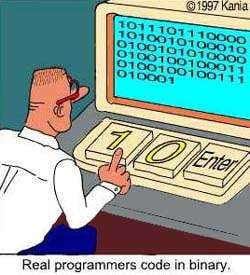
\includegraphics[width=0.8\textwidth]{images/real-programmers-binary.jpg}
  \caption{Справжні розробники кодують програми у бінарному режимі.}
  \label{PicRealDevelopers}
\end{figure}

\begin{figure}
  \centering
  \begin{subfigure}[b]{0.45\textwidth}
    \centering
    
\includegraphics[width=\textwidth]{images/qr2.png}
    \caption{~}
    \label{Pic_QR_BW}
  \end{subfigure}
  \hfill
  \begin{subfigure}[b]{0.45\textwidth}
    \centering
    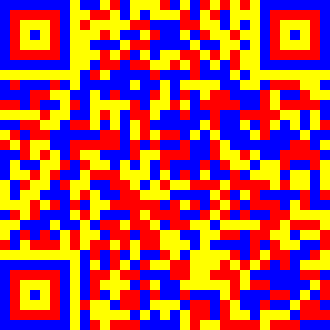
\includegraphics[width=\textwidth]{images/qr3.png}
    \caption{~}
    \label{Pic_QR_Color}
  \end{subfigure}
  \caption{На QR коді ми можемо на власні очі побачити біти (а); також показаний гіпотетичний QR код, який складається зі тритів (б).}
  \label{PicQR}
\end{figure}

Але я б хотів виділити один момент, який буде для нас важливим, та на якому я хотів би побудувати розповідь.
Інформація це часто є акцентування aбо позначення однієї з можливих альтернатив.
Наприклад, «Танєєв народився у 1856 році».\footnote{
  Приклад про Танєєва взятий з оповідання Іраклія Андронікова «Перший раз на естраді», яке можна прочитати в інтернеті або подивитися на youtube.
  \par\url{https://www.youtube.com/watch?v=dm8wdFKag94}}
Це означає, що Танєєв не міг народитися у 1858 році, 1859, 1860, 1861, 1862, і т.~д.
Тобто з усіх можливих альтернатив, коли міг народитися Танєєв, ми обираємо одну.
Цього погляду нам вистачить для потреб цієї книги.

Добре, тепер спробуємо поміркувати так, як це роблять програмісти та математики.
Який шмат інформації самий найпростіший?
Інтуїтивно, це вибір однієї з двох альтернатив.
Тому що три це вже забагато, а у разі однієї альтернативи мова не йде про вибір.
«Танєєв народився від батька та матері!»
Це викликає посмішку, бо незрозуміло, які є ще варіанти?
Так, з сучасними технологічними досягненнями у галузі біомедицини, у певному контексті ще можна уявити на чому саме робиться акцент, але не у 1856 році.

Сама дрібна одиниця інформація, а саме вибір однієї з двох альтернатив, називається бітом. \index{біт}
Це може бути орел чи решка, парне або непарне, біле або чорне, хрестик або нулик, \Male\ або \Female, живий або мертвий, уперед чи назад, правда чи брехня.

\begin{exercise}
Придумайте ще приклади інформації, які можна закодувати одним бітом.
\end{exercise}

У сучасній мікроелектроніці, біт це наявність або відсутність електричного сигналу за певний проміжок часу, який називається тактом. \index{такт}
Переважна кількість сучасних процесорів бачать увесь свій світ виключно як послідовність біт.
Коли ми на комп'ютері слухаємо музику, дивимося відео або граємо у 3D ігри, коли робиться автоматичний переклад з однієї мови на іншу, коли автоматично генеруються пейзажі, то інколи дуже важко повірити в те, що віртуальна реальність складається виключно з бітів, але це так.
Однією нашою метою буде як раз пояснення того, як реальний світ може бути змодельований з бітів.

Проте, поширення електронних пристроїв призвело до того, що ми можемо фізично побачити біти навіть у реальному житті.
Гарний приклад цього це QR~коди, де біти видно на власні очі (рис.~\ref{Pic_QR_BW}).
Тут чорні квадратики кодують один стан, а білі---інший.

Оскільки ми будемо вести багато розмов про біти, треба їх якось позначати.
Біт може бути у одному з двох станів, для цього можна вибрати два будь-яких символи, наприклад $\blacksquare$ та $\square$, як на QR~коді.
Але історично в математиці використовуються числа $0$ та $1$.
Щоб відрізняти звичайні десяткові числа, складені з нулів та одиниць, наприклад, як  $101$ (сто один),  від послідовності біт \bitstr{1}, \bitstr{0} та \bitstr{1}, ми будемо триматися наступних домовленостей:
\bitdesc

За визначенням, один біт може кодувати два різних варіанти. А скільки варіантів кодує два біти? Нескладно порахувати, що відповідь на це запитання буде чотири, ось усі варіанти: \bitstr{00}, \bitstr{01}, \bitstr{10} та \bitstr{11}. Взагалі, якщо ми збільшуємо кількість біт на один, то кількість варіантів зростає у двічі.
Це легко пояснити тим, що для будь якого попередньої комбінації ми можемо додати або біт \bitstr{0}, або біт \bitstr{1}.
Загально, якщо в нас є $n$ біт, то з них можна скласти $2^n$ різних комбінацій.

\begin{exercise}
Побудуйте усі різні комбінації, які можна створити з трьох біт.
\end{exercise}

\begin{exercise}
Скільки усього можливих комбінацій можна скласти з $10$ біт?
\end{exercise}

Я сподіваюся, що до цього моменту ви вже розібралися, що таке біти.
Тому настав час трохи відпочити та пофлудити.
Отже, біт має два стани, які ми позначаємо \bitstr{0} та \bitstr{1}.
Також ми відмітили, що безглуздо розглядати щось, що має лише один стан.
А якщо розглянути систему, яка має три стани, наприклад \tritzero, \tritone\ та \trithalf?
\index{тріт} Назвемо трітом одиницю інформації, де у нас є вибір з трьох альтернатив.

\begin{exercise}
Побудуйте усі різні комбінації, які можна створити з двох тритів.
\end{exercise}

Чи дасть це нам якісь переваги?
З математичної точки зору, усе що можна представити з тритів, можна представити й за допомогою бітів.
Самий простий шлях це зробити просто використовувати два біти для кодування одного тріта: \bitstr{00}~—~\tritzero, \bitstr{11}~—~\tritone\ та \bitstr{01}~—~\trithalf.
Так, звичайно комбінація \bitstr{10} не буде використовуватися.
Так, звичайно бітів буде вдвічі більше ніж тритів.
Але коли це хвилювало математиків?

\begin{exercise}
Скільки біт треба для того, щоб закодувати інформацію, яка міститься у двох трітах?
Скільки комбінацій при цьому не буде використано?
\end{exercise}

Добре, а що з точки зору народного господарства?
Якщо зберігати інформацію у трітах замість бітів, чи не виграємо ми додаткове місце?
Яке не яке, а досягнення.
Але, на практиці усе не так просто.
Безкоштовний газ є тільки у газовій камері.

Подивимося на рис.~\ref{Pic_QR_Color}.
На ньому я намагався нафантазувати, як би мав виглядати QR~код з тритів.
Замість чорної та білої фарб, використано жовту, синю та червоні фарби.
Ніби то виграш є?
Але на практиці розрізняти три фарби складніше.
Тому у звичайному чорно-білому варіанті ми зможемо розрізняти менші квадратики, а це також буде впливати на щільність запису інформацію.

Зробити процесори, які працюють з трітами, не питання.
За радянських часів була побудована ЕОМ Сетунь\footnote{\setunref}, яка працювала з трітами. \index{Сетунь}
Розрізнялися не тільки наявність та відсутність сигналу, але й його напрямок.
Хтось й по сьогоднішній день вважає це революційним досягненням, але я до цього ставлюся скептично.
Проектування процесорів зараз суто технічний процес.
Е багато інструментів, програмних застосунків, які дозволяють моделювати нові процесори.
Цим займається багато спеціалістів по усьому світу, тому усе що можна було перепробувати, вони вже перепробували.
Отже, якщо переважна більшість сучасних комп'ютерів працюють з бітами, то це означає, що не зважаючи на свою привабливість, тріти все ж таки програють бітам.

Але, там де це доречно, то чому б не розглянути?
У WiFi інформація передається символами, кожен з яких може нести величезну кількість варіантів.
Так, оскільки ця інформація у евентуально буде оброблятися звичайним процесором, то з практичної точки зору цю кількість варіантів намагаються зробити ступенями двійки.
Це дає змогу казати, що один символ несе $1024$ біти інформації.
Але у самій електромагнітній хвилі важко побачити окремі біти.

Також скажу декілька слів про квантові обчислення, кубіти, або квантові біти. \index{кубіт}
Так, на сьогодні віртуальний світ складається з бітів. А що у реальному?
Якщо опуститися на рівень квантових взаємодій, ми побачимо, що там працюють свої екзотичні контрінтуїтивні закони.
Окрім двох альтернатив, які виключають одна одну, ми часто бачимо їх суперпозицію.
Наприклад, електрон на $30$\% обертається праворуч, а на $70$\%---ліворуч.
Нам це важко уявити, але математичні формули працюють саме так.
Замість нуля та одиниці, ми отримуємо фізичну величину від нуля до одиниці.
Додайте ще фазу від нуля до $2\pi$, й ви отримаєте кубіт.
А ще суперпозиція станів, зворотні операції, вимірювання...

Вже з'являються перші квантові комп'ютери, які оперують кубітами.
Це може бути новою революцією.
Але на початку все ж таки краще освоїти звичайне програмування, яке працює з бітами.
А вже потім переходити до квантового.

\begin{exercise}
Продивиться статтю у Wikiepedia про квантові комп'ютери\footnote{\quantumref}. Чи це цікаво?
\end{exercise}

\begin{summary}
\item Інформація вимірюється у бітах.  Біт це найменший шмат інформації, який складається з двох станів, які позначаються \bitstr{0} та \bitstr{1}.
\item З $n$ біт можна скласти $2^n$ різних комбінацій.
\end{summary}

\section{Числа, скільки біт нам вистачить?}

Відомий німецький математик Леопольд Кронекер якось казав: «Бог створив натуральні числа, решта — справа рук людини».
Числа відіграють дуже важливу роль в нашому житті, тому розглянемо, як можна складати з біт натуральні числа.
Але, на превеликий жаль, точна відповідь на це запитання «Ніяк».
Натуральних чисел нескінченна кількість, тому скільки би ми не брали бітів, все одно з них можна буде скласти лише обмежену кількість різних комбінацій.

Але, якщо підійти до цієї проблеми не з точки зору теорії, а з боку потреб народного господарства, то як часто ми маємо проблему працювати з величезними числами?
Як часто у повсякденному житті ми чуємо про квадрильйони, та секстильйони?

\begin{exercise}
Скільки нулів наприкінці в записі чисел «один квадрильйон» та «один секстильйон»?
\end{exercise}

Тому заслуговує уваги практичний спосіб вирішення проблеми, коли ми кодуємо не усі натуральні числа, а до деякого числа, яке нам здається розумним обмеженням.
Якщо для збереження натурального числа виділити $n$ біт, то, як ми вже знаємо, ми зможемо зберігати $2^n$ різних комбінацій.
Оскільки перше число, яке ми будемо зберігати, це $0$, то останнє число буде $2^n-1$.
Оцінимо тепер різні значення $n$, які часто зустрічаються на практиці.

Припустимо, $n=8$. Як ми дізнаємося пізніше, це байт.
Таким чином ми можемо зберігати числа від $0$ до $255$.
Такий діапазон покриває лише невеличку частину потреб.
Наприклад, у восьмі бітах ми можемо зберігати кількість дітей, пульс (кількість ударів за хвилину), кількість сторінок у зошиті, кількість кнопок у миші, і~т.~д.
Але для зберігання більшості чисел, з якими ми зустрічаємося на практиці, цього буде недостатньо.

\begin{exercise}
Приведіть приклади значень, для зберігання яких достатньо восьмі біт.
\end{exercise}

У $2010$-х роках була популярна $32$-бітна архітектура.
Цієї кількості біт вистачає для збереження чисел від $0$ до $4~294~967~295$.
Цього вже достатньо для багатьох практичних потреб, будь то заробітна платня або кількість книг у бібліотеці.
Але все ж таки існують й виключення, наприклад борг державного департаменту США, або населення земної кулі.

\begin{exercise}
Наведіть приклади значень, для збереження яких нам не вистачить $32$-х біт.
\end{exercise}

Тут може виникати запитання, можемо чи ми працювати з $64$-х, або навіть з $128$-ми бітними числами, якщо у нас $32$-бітний процесор.
Відповідь на це запитання проста: можемо, але це буде повільніше.
Бітність процесора означає, над якими числами дії будуть виконуватися за одну операцію.
Щоб працювати з числами з більшою кількістю бітів, нам треба буде написати або використати готові програми, які будуть виконувати потрібні дії але за більшу кількість елементарних операцій.

Зараз більшість комп'ютерів має $64$-бітну архітектуру, таким чином діапазон складає від $0$ до запаморочливого числа $18~446~744~073~709~551~615$, яке вимовляється «18 квінтильйонів, 446 квадрильйона, ...»
Як часто у житті ви оперуєте такими числам? Особисто я не часто.
Цікаво, що це число з'являється у притчі про раджу та винахідника шахів, який у нагороду попросив трохи зерна, одне на першу клітину, два на другу, чотири на третю,~...
На шахівниці усього $64$ клітини, тому  не дивно, що ці числа збіглися.

Але це ще не кінець.
Розробники криптовалюти Ethereum, платформи для смарт-контрактів, вибрали для своєї архітектури $512$ біт.\index{Ethereum}
Цього достатньо, щоб зберігати числа, які складаються зі $150$-ти цифр, а це більше ніж гугол, число $1^{100}$ або одиниця та сто нулів!
Вибір такого числа пояснюється тим, що зробити підтримку для мікротранзакцій з сумами значно менше ніж один цент.
$1$~wei, найдрібніше значення криптовалюти ETH, яким можна оперувати, на момент написання книги коштувало $0.000~000~000~000 002~598$ доларів.
Але головною причиною вибору такого значення був все ж таки технічний момент.
Автори Ethereum вибрали алгоритм хешування, який повертає $512$-бітне число.

Скажемо пару слів про хешування, та чому саме для нього потрібні такі величезні числа.\index{хеш}
Алгоритм хешування полягає у тому, щоб задану послідовність біт перетворити у певне обмежене число, яке називається хешем цієї послідовності.
Хешування є криптографічним, якщо \textit{практично неможливо}\footnote{
  Це означає, що сьогодні ніхто не наблизився до розв'язку цієї задачі.
  Або, якщо використовувати сучасні алгоритми, та усю планету перетворити на велетенський процесор, то потрібні будуть квінтильйони років для розв'язку.
} по хешу знайти послідовність біт, з якого він був згенерований, чи згенерувати дві послідовності, яким буде відповідати один й той самий хеш.
Таким чином, наприклад, дві сторони можуть опублікувати, що вони підписали договір, та надати його хеш.
Тоді ніхто не буде знати, який саме договір підписали сторони.
Але кожна зі сторін, наприклад у разі виникнення спору, може показати у суді договір, який відповідає хешу.
Ця техніка зазвичай дуже важлива для блокчейна.
Але якщо вибрати у якості хешу $32$-бітне число, то можна просто перебрати трохи більше $4$~млрд. різних послідовностей та знайти дві з однаковим хешем.
%Здається що перебрати таку кількість варіантів надзвичайно складна робота, але сучасні процесори можуть з цим впоратися.
Чим більше біт, тим складніше перебирати та знаходити слабкі місця у алгоритмі.
Як раз $256$ та $512$-бітні хеші на сьогодні є компромісом між безпекою та швидкодією.

Далі йдуть цифрові підписи та шифрування.
Там компроміс між безпекою та швидкодією приводить нас до $1024$ або $2048$-бітного шифрування.
Але й інколи в деяких країнах у це втручається навіть закон, який обмежує кількість біт, які мають використовуватися для шифрування.
Напевне, щоб влада могла розшифрувати, якщо їй дуже сильно закортить.

Добре, припустимо ми виділили із запасом мільйон біт.
Думаєте цього усім вистачить?
Помиляєтеся, та дуже недооцінюєте математиків!
Вони дійшли до таких чисел, що навіть якщо для виділити усі диски у світі, все рівно їх не вистачить для зберігання навіть одного числа!
Прикладом такого числа є $TREE(3)$ з теореми Крускала\footnote{\kruskalref}.

\begin{summary}
\item Натуральних чисел нескінчена кількість, тому на практиці обмежуються деяким числом, яке, здається, неможливо перебільшити.
\item Чим більше біт використовується, тим більше потреб покривається, але тим повільніші операції. $64$-біт вистачає для більшості потреб.
\item Математики---божевільні!
\end{summary}

\section{Як скласти числа з біт?}

Добре, ми трохи обговорили тему, скільки біт треба виділити на числа у разі тієї чи іншої задачі.
Тепер треба вирішити більш практичне запитання: «Яким методом можна скласти числа з біт?» (рис.~\ref{Pic_Num_From_Bits})

\afterpage{
\begin{figure}[t]
  \centering
  \begin{tikzpicture}
  % \draw[help lines] (0,0) grid (7,3);

  \node at (0.5,2.8) {$0$};
  \node at (1.0,2.8) {$1$};
  \node at (1.5,2.8) {$2$};
  \node at (2.0,2.8) {$3$};
  \node at (2.5,2.8) {$4$};
  \node at (3.0,2.8) {$5$};
  \node at (3.5,2.8) {$6$};
  \node at (4.0,2.8) {$7$};

  \node at (0.6, 0.2) {\bitstr{000}};
  \node at (1.6, 0.2) {\bitstr{001}};
  \node at (2.6, 0.2) {\bitstr{010}};
  \node at (3.6, 0.2) {\bitstr{100}};
  \node at (4.6, 0.2) {\bitstr{011}};
  \node at (5.6, 0.2) {\bitstr{101}};
  \node at (6.6, 1.0) {\bitstr{110}};
  \node at (6.6, 1.8) {\bitstr{111}};

  \draw (0.5,2.65)
    to [out=-90,in=180] (2.5, 0.7)
    to [out=0,in=-135] (3.5, 1.5)
    ;

  \draw (1.0,2.65)
    to [out=-90,in=180] (2.5, 2)
    to [out=0,in=135] (3.5, 1.5)
    ;

  \draw (1.5,2.65)
    to [out=-90,in=180] (2.8, 1.0)
    to [out=0,in=180] (3.5, 1.5)
    ;

  \draw (2.0,2.65)
    to [out=-90,in=180] (2.8, 1.8)
    to [out=0,in=180] (3.5, 1.5)
    ;

  \draw (2.5,2.65)
    to [out=-90,in=180] (3.0, 1.6)
    to [out=0,in=-135] (3.5, 1.5)
    ;

  \draw (3.0,2.65)
    to [out=-90,in=-90] (3.5, 1.5)
    ;

  \draw (3.5,2.65)
    to [out=-90,in=-90] (3.5, 1.5)
    ;

  \draw (4.0,2.65)
    to [out=-90,in=-80] (3.5, 1.5)
    ;

  \draw (0.6,0.35)
    to [out=90,in=180] (1.5, 1.8)
    to [out=0,in=-170] (3.5, 1.5)
    ;

  \draw (1.6,0.35)
    to [out=90,in=170] (2.5, 1.4)
    to [out=0,in=-150] (3.5, 1.5)
    ;

  \draw (2.6,0.35)
    to [out=90,in=-166] (3.5, 1.5)
    ;

  \draw (3.6,0.35)
    to [out=90,in=-90] (3.5, 1.5)
    ;

  \draw (4.6,0.35)
    to [out=90,in=-60] (3.5, 1.5)
    ;

  \draw (5.6,0.35)
    to [out=90,in=-30] (3.5, 1.5)
    ;

  \draw (6.3,1.0)
    to [out=180,in=10] (3.5, 1.5)
    ;

  \draw (6.3,1.8)
    to [out=180,in=30] (3.5, 1.5)
    ;

  \draw [fill=white] (3.5,1.5) circle [radius=0.5];
  \node at (3.5, 1.5) {?};

\end{tikzpicture}

  \caption{Яким саме послідовностям біт мають відповідати числа?}
  \label{Pic_Num_From_Bits}
\end{figure}
}

Знову, як математики та програмісти, на початку спробуємо розглянути самий елементарний випадок, а саме один єдиний біт.
Отже, у нас $n=1$, у нас є послідовності \bitstr{0} та \bitstr{1}.
Нам треба зіставити цим послідовностям числа $0$ та $1$.
Яким чином це можна зробити?
Сподіваюся, що якщо ви не диверсант, то вибрали природній шлях нуль назвати нулем, а одиницю---одиницею.

Тепер спробуємо розглянути випадок $n=2$.
Тепер ми маємо послідовності \bitstr{00}, \bitstr{01}, \bitstr{10}, \bitstr{11}, та числа $0$, $1$, $2$, $3$.
Тут гарно пригадати властивості звичайних чисел, а саме що до будь-якого числа можна зліва приписати будь яку кількість нулів, воно від цього не зміниться: $42 = 042 = 00042$.
Це дуже зручно на практиці, бо не треба гадати, як число з чотирьох біт перевести у число з восьми бітами: просто дописуємо потрібну кількість нулів.
Таким чином, ми вже маємо, що \bitstr{00} це $0$, а \bitstr{01} це $1$.
Лишилося лише знайти відповідність між \bitstr{10} й \bitstr{11}, ти числами $2$ і $3$.

І знову два способи це зробити: перший, коли $2$ це \bitstr{10}, а $3$ це \bitstr{11}; та другий, коли $2$ це \bitstr{11}, а $3$ це \bitstr{10}.
Якщо придивитися, то ми обидва рази приписуємо зліва одиницю, тут ніякого вибору в нас немає.
Але, якщо не звертати на її увагу, то перший раз буде \bitstr{0}, \bitstr{1}, тобто та послідовність, яку ми вже отримали при $n=1$.
Другий раз ми приписуємо зліва одиницю до \bitstr{1}, \bitstr{0}, тобто ми записали послідовність, яка була при $n=1$, але задом-наперед.
Звичайно, що перша спроба здається нам більш простішою та логічною: менше зайвих рухів.
Так, цей метод дає нам двійкову систему числення, яка й використовується у переважної більшості сучасної електроніки.\index{система числення, двійкова}
Але й зворотній порядок не безглуздий, таким чином утворюється кодування Грея, яка інколи має свої переваги.\index{Грея, кодування}

Сконцентруємося спочатку на двійковій системі числення.
Спробуємо описати більш формально послідовність кроків, як побудувати цю послідовність для будь-якого числа біт.
Коли математики кажуть «більш формально», то це означає, що опис містить менше натяків, котрі кожен може зрозуміти на власний розсуд.\index{формальний опис}
Наприклад, візьмемо послідовність дій з реального життя, наприклад «піди купи молоко».
Більше формальний опис буде: «Вийди з дому, прямуй по вулиці Гоголя на північ, через $200$~метрів, там буде магазин Гастроном, у якому купи молоко~$3.5$\% жиру.»
Зазвичай, написання програм, яке ми мріємо опанувати,  це перекладення побажань користувача на формальну мову програмування.

Якщо опис для вирішення задачі настільки формальний, його може виконати навіть механічний пристрій (читаємо комп'ютер), то ми його називаємо алгоритмом.\index{алгоритм}
У нашому випадку ми отримуємо:

\begin{algorithm}
  \algcaption{Побудова послідовності у двійковій системі числення}
  \alginput{Вже побудована послідовність $A$ для $n$ біт}
  \algoutput{Продовжити послідовність для $n+1$ біт}
  \begin{algsteps}
    \algstep Виписати послідовність $A$.
    \algstep Для кожного елементу щойно виписаної послідовності приписати зліва нуль.
    \algstep Виписати ще раз послідовність $A$.
    \algstep Для кожного елементу щойно виписаної послідовності приписати зліва одиницю.
  \end{algsteps}
  \algsummary{У нас буде виписана послідовність для $n+1$ біт}
\end{algorithm}

Тепер спробуємо розібратися, як працює цей алгоритм.
На початку розглянемо випадок $n=1$, та спробуємо ретельно виконати кожен крок.
Отже, самий початок, нам треба вже побудована послідовність для одного біта.
Ми вже розглядали цей випадок, такою послідовністю буде \bitstr{0}, \bitstr{1}.
Запам'ятали, що це буде наше $A$.

Перший крок полягає у тому, щоб виписати цю послідовність.
Це нескладно, у нас послідовність $A$ складається в двох елементів:
\par\bitstr{~~~~~0~~1}\par
Другий крок---приписати зліва нуль до кожного елементу послідовності.
Що ж, приписуємо:
\par\bitstr{~~~~00~01}\par
Третій крок, нам треба знову виписати послідовність $A$, яка складається з двох елементів.
Виписуємо:
\par\bitstr{~~~~00~01~~0~~1}\par
Четвертий крок---приписати до щойно виписаних двох елементів зліва одиницю.
Робимо й це:
\par\bitstr{~~~~00~01~10~11}\par
Вуаля, ми дійшли до кінця, та ми отримали послідовність з чотирьох елементів \bitstr{00}, \bitstr{01}, \bitstr{10}, \bitstr{11}.
Це й буде послідовність чисел у двійковій системі числення для $n=2$.
Завдання виконано!

\begin{exercise}
А тепер відкладіть цю книгу, та повторіть усі ці кроки самостійно. Перечитайте ще раз, якщо є певні непорозуміння.
\end{exercise}

Тепер розглянемо випадок $n=2$.
Ми щойно побудували двобітові послідовності для двійкової системи числення.
Наступна наша мета це перейти від щойно отриманого результату до трьохбітових послідовностей.
Якщо ретельно виконувати кожен крок нашого алгоритму, ми отримаємо наступні результати після кожного кроку:

\par\bitstr{~~~~~00~~01~~10~~11}\par
\par\bitstr{~~~~000~001~010~011}\par
\par\bitstr{~~~~000~001~010~011~~00~~01~~10~~11}\par
\par\bitstr{~~~~000~001~010~011~100~101~110~111}\par

\begin{exercise}
Виконати наш алгоритм для $n=3$ для отримання чотирьохбітових послідовностей.
\end{exercise}

\begin{exercise}
Нехай загнутий палець відповідає цифрі \bitstr{0}, а відігнутий---цифрі \bitstr{1}.
Спробуйте порахувати на пальцях однієї руки від $0$ до $31$ у двійковій системі числення.
\end{exercise}

Наприкінці декілька слів про кодування Грея.
Пригадаємо, що ми казали, що цей зворотній порядок не безглуздий.
Спробуємо змінити наш алгоритм таким чином, щоб він будував числа у кодуванні Грея.
Як ми казали, другий раз треба виписувати нашу послідовність у зворотньому порядку.
Таким чином, у нашому алгоритмі зміниться лише третій крок:

\begin{algorithm}
  \algcaption{Побудова послідовності біт у кодуванні Грея}
  \alginput{Вже побудована послідовність $A$ для $n$ біт}
  \algoutput{Побудувати послідовність для $n+1$ біт}
  \begin{algsteps}
    \algstep Виписати послідовність $A$, яка у нас уже є
    \algstep Приписати зліва нуль
    \algstep Виписати задом наперед послідовність $A$
    \algstep Приписати зліва одиницю для щойно виписаної послідовності
  \end{algsteps}
\end{algorithm}

Таким чином, для $n=2$ результат виконання алгоритму після кожного кроку буде виглядати наступним чином:
\par\bitstr{~~~~~0~~1}\par
\par\bitstr{~~~~00~01}\par
\par\bitstr{~~~~00~01~~1~~0}\par
\par\bitstr{~~~~00~01~11~10}\par

А це випадок для $n=3$:
\par\bitstr{~~~~~00~~01~~11~~10}\par
\par\bitstr{~~~~000~001~011~010}\par
\par\bitstr{~~~~000~001~011~010~~10~~11~~01~~00}\par
\par\bitstr{~~~~000~001~011~010~110~111~101~100}\par

Єдина складність полягає у тому, щоб не заплутатися та не узяти якийсь результат з алгоритму для двійкової системи числення, або не забути на третьому кроці про слова «задом-наперед».

\begin{exercise}
Побудувати коди Грея для чотирьох біт.
\end{exercise}

Добре, а чим саме корисне кодування Грея?
Це досить специфічне питання більше для загальної освіти, ніж для практичного застосування.
Але, як на мене, цікаве.
Порівняємо, як відбувається перехід від числа $3$ до числа $4$ у двійковій системі числення, та у кодуванні Грея.

\par$3 \to 4$: \bitstr{~~~~~~011} $\to$ \bitstr{100} (двійкова система)
\par$3 \to 4$: \bitstr{~~~~~~010} $\to$ \bitstr{110} (кодування Грея)

Ми бачимо, що у двійковій системі числення кожен біт змінив своє значення.
Самий лівий був \bitstr{1}, а став \bitstr{0}.
Середній також був \bitstr{1} й також став \bitstr{0}.
А самий правий біт, навпаки, був \bitstr{0}, а став \bitstr{1}.

У кодуванні Грея помінявся лише самий правий біт, був \bitstr{0}, а став \bitstr{1}.
Лівий та середній біти на змінилися.
Це є як раз і є корисна властивість кодування Грея: коли ми переходимо до наступного числа, у нас змінюється значення рівно один біту.

\begin{exercise}
Перевірте цю властивість для послідовності трьохбітових кодів Грея: \bitstr{000~001~011~010~110~111~101~100}.
\par Підкресліть ті біти, які змінять своє значення у наступному числі.
\end{exercise}

\begin{figure}[tb]
  \centering
  \pgfmathsetmacro{\ticksz}{0.4}
\pgfmathsetmacro{\ltick}{1.1}
\pgfmathsetmacro{\rtick}{1.4}
\pgfmathsetmacro{\W}{2.5}

\begin{subfigure}[b]{0.45\textwidth}
  \centering
  \begin{tikzpicture}
      \draw (0.6,0) to ({\W},0);
      \draw [dashed] (0.6,{1*\ticksz}) to ({\W},{1*\ticksz});
      \draw [dashed] (0.6,{2*\ticksz}) to ({\W},{2*\ticksz});
      \draw [dashed] (0.6,{3*\ticksz}) to ({\W},{3*\ticksz});
      \draw [dashed] (0.6,{4*\ticksz}) to ({\W},{4*\ticksz});

      \node at (0.1, {0*\ticksz}) {$0$ м};
      \node at (0.1, {1*\ticksz}) {$1$ м};
      \node at (0.1, {2*\ticksz}) {$2$ м};
      \node at (0.1, {3*\ticksz}) {$3$ м};
      \node at (0.1, {4*\ticksz}) {$4$ м};

      \node at ({\W}, {0.5*\ticksz}) {\bitstr{00}};
      \node at ({\W}, {1.5*\ticksz}) {\bitstr{01}};
      \node at ({\W}, {2.5*\ticksz}) {\bitstr{10}};
      \node at ({\W}, {3.5*\ticksz}) {\bitstr{11}};

      \draw [ultra thick] ({\ltick},{2*\ticksz}) to ({\ltick},{4*\ticksz});
      \draw [ultra thick] ({\rtick},{1*\ticksz}) to ({\rtick},{2*\ticksz});
      \draw [ultra thick] ({\rtick},{3*\ticksz}) to ({\rtick},{4*\ticksz});

  \end{tikzpicture}
  \caption{~}
\end{subfigure}
\hfill
\begin{subfigure}[b]{0.45\textwidth}
  \centering
  \begin{tikzpicture}
      \draw (0.6,0) to ({\W},0);
      \draw [dashed] (0.6,{1*\ticksz}) to ({\W},{1*\ticksz});
      \draw [dashed] (0.6,{2*\ticksz}) to ({\W},{2*\ticksz});
      \draw [dashed] (0.6,{3*\ticksz}) to ({\W},{3*\ticksz});
      \draw [dashed] (0.6,{4*\ticksz}) to ({\W},{4*\ticksz});

      \node at (0.1, {0*\ticksz}) {$0$ м};
      \node at (0.1, {1*\ticksz}) {$1$ м};
      \node at (0.1, {2*\ticksz}) {$2$ м};
      \node at (0.1, {3*\ticksz}) {$3$ м};
      \node at (0.1, {4*\ticksz}) {$4$ м};

      \node at ({\W}, {0.5*\ticksz}) {\bitstr{00}};
      \node at ({\W}, {1.5*\ticksz}) {\bitstr{01}};
      \node at ({\W}, {2.5*\ticksz}) {\bitstr{11}};
      \node at ({\W}, {3.5*\ticksz}) {\bitstr{10}};

      \draw [ultra thick] ({\ltick},{2*\ticksz}) to ({\ltick},{4*\ticksz});
      \draw [ultra thick] ({\rtick},{1*\ticksz}) to ({\rtick},{3*\ticksz});
  \end{tikzpicture}
  \caption{~}
\end{subfigure}

  \caption{Прилад, датчики якого повертають значення у (а) двійковому кодуванні; (б) кодуванні Грея.}
  \label{Pic_Device}
\end{figure}

Ця властивість буде нам у нагоді, коли кожен біт це результат окремого вимірювання.
Припустимо, що ми будуємо прилад, який вимірює відстань до деякого об'єкту та повертає $0$, $1$, $2$ або $3$ метри (рис.~\ref{Pic_Device}).

Для двійкової системи (а), датчик, що відповідає за лівий біт, має повертати значення \bitstr{1}, якщо відстань більше за $2$ метри.
А датчик, що відповідає правий біт, має повертати значення \bitstr{1} якщо відстань знаходиться від $1$ до $2$ метрів, або більше ніж $3$ метри.
Проблема полягає у тому, що на практиці, на жаль, неможливо побудувати датчик, який буде повертати точне значення без помилок.

\begin{figure}[t]
  \centering
  \pgfmathsetmacro{\ticksz}{0.4}
\pgfmathsetmacro{\ltick}{1.5}
\pgfmathsetmacro{\rtick}{2.1}
\pgfmathsetmacro{\W}{3.5}

\begin{tikzpicture}
  \node at (0,{0.5*\ticksz}) {$1.95$ м};
  \node at (0,{1.5*\ticksz}) {$1.96$ м};
  \node at (0,{2.5*\ticksz}) {$1.97$ м};
  \node at (0,{3.5*\ticksz}) {$1.98$ м};
  \node at (0,{4.5*\ticksz}) {$1.99$ м};
  \node at (0,{5.5*\ticksz}) {$2.00$ м};
  \node at (0,{6.5*\ticksz}) {$2.01$ м};
  \node at (0,{7.5*\ticksz}) {$2.02$ м};
  \node at (0,{8.5*\ticksz}) {$2.03$ м};
  \node at (0,{9.5*\ticksz}) {$2.04$ м};

  \draw [dashed] (0.7,{0.5*\ticksz}) to ({\W},{0.5*\ticksz});
  \draw [dashed] (0.7,{1.5*\ticksz}) to ({\W},{1.5*\ticksz});
  \draw [dashed] (0.7,{2.5*\ticksz}) to ({\W},{2.5*\ticksz});
  \draw [dashed] (0.7,{3.5*\ticksz}) to ({\W},{3.5*\ticksz});
  \draw [dashed] (0.7,{4.5*\ticksz}) to ({\W},{4.5*\ticksz});
  \draw          (0.7,{5.5*\ticksz}) to ({\W},{5.5*\ticksz});
  \draw [dashed] (0.7,{6.5*\ticksz}) to ({\W},{6.5*\ticksz});
  \draw [dashed] (0.7,{7.5*\ticksz}) to ({\W},{7.5*\ticksz});
  \draw [dashed] (0.7,{8.5*\ticksz}) to ({\W},{8.5*\ticksz});
  \draw [dashed] (0.7,{9.5*\ticksz}) to ({\W},{9.5*\ticksz});

  \node at ({\ltick}, -0.4) {Л};
  \node at ({\rtick}, -0.4) {П};

  \draw [ultra thick] ({\ltick},{10*\ticksz}) to ({\ltick},{3*\ticksz});
  \draw [ultra thick] ({\rtick},{0*\ticksz}) to ({\rtick},{7*\ticksz});

  \node [right] at ({1.1*\W},{0.5*\ticksz}) {\bitstr{01~~~} $1$ м};
  \node [right] at ({1.1*\W},{1.5*\ticksz}) {\bitstr{01~~~} $1$ м};
  \node [right] at ({1.1*\W},{2.5*\ticksz}) {\bitstr{01~~~} $1$ м};
  \node [right] at ({1.1*\W},{3.5*\ticksz}) {\bitstr{11~~~} $3$ м  ???};
  \node [right] at ({1.1*\W},{4.5*\ticksz}) {\bitstr{11~~~} $3$ м  ???};
  \node [right] at ({1.1*\W},{5.5*\ticksz}) {\bitstr{11~~~} $3$ м  ???};
  \node [right] at ({1.1*\W},{6.5*\ticksz}) {\bitstr{11~~~} $3$ м  ???};
  \node [right] at ({1.1*\W},{7.5*\ticksz}) {\bitstr{10~~~} $2$ м};
  \node [right] at ({1.1*\W},{8.5*\ticksz}) {\bitstr{10~~~} $2$ м};
  \node [right] at ({1.1*\W},{9.5*\ticksz}) {\bitstr{10~~~} $2$ м};
\end{tikzpicture}

  \caption{Проблема зона у приладі, датчики якого повертають значення у двійковому кодуванні.
           Літерою Л позначено датчик, що відповідає за лівий біт, а літерою П---за правий.}
  \label{Pic_DeviceError}
\end{figure}

Давайте поміркуємо, що буде у випадку, коли значення повертаються з помилками.
Припустимо, що у реальному світі датчик, що відповідає за лівий біт (позначимо його Л), повертає значення \bitstr{1} коли відстань більше ніж $1.98$ метри.
А датчик, що відповідає за правий біт (П), буде повертати \bitstr{1} коли відстань потрапляє у діапазон від $1.02$ до $2.01$ метрів, або більше ніж $3.03$ метри.
Що буде відбуватися, коли відстань буде коливатися біля двох метрів?
Відповідь на це дає рис.~\ref{Pic_DeviceError}.
Ми бачимо, що коли відстань до об'єкту потрапляє у діапазон від $1.98$ до $2.01$ метри, наш прилад повертає значення $3$~м, або \bitstr{11} у двійковій системі.
Можна сказати, що це значення «ніяк не пов'язано з реальністю, простіше кажучи «від балди».
Такі проблеми досить важко вирішувати.

\begin{exercise}
Нарисуйте аналог рисунку~\ref{Pic_Device} для датчика з трьома бітами замість двох.
\end{exercise}

\begin{exercise}
Нарисуйте аналог рисунку~\ref{Pic_DeviceError} для кодування Грея на відстані біля $2$~м, та переконайтеся, що там ця проблема не виникає.
\end{exercise}

\begin{exercise}
Це був важкий параграф, де ви могли дізнатися багато нових речей. Тому зараз дуже гарний привід, щоб трохи відпочити та випити свого улюбленого напою.
\end{exercise}

\begin{exercise}
Відпочили? Знову з нуля побудуйте послідовності у двійковій системі числення та у кодування Грея. Нічого не забули?
\end{exercise}

\begin{summary}
\item Числа з бітів можна складати різними способами.
\item Найпоширеніший спосіб це двійкове кодування.
\item Ще один екзотичний спосіб це кодування Грея.
\item Алгоритм це формальна послідовність кроків, для досягнення певної мети.
\item Людина має виконувати алгоритми виключно спинним мозком.
\end{summary}

\section{Системи числення}

У попередньому параграфі ми дізналися про те, що таке двійкова система числення.
Звичайні числа, на кшталт $42$ та $1024$, це десяткова система числення.\index{система числення, десяткова}
Тобто, дві системи числення вже знаємо.
Тепер настав час узагальнення, поговоримо про системи числення за будь якою основою $n$.\index{основа системи числення}

Але розпочнемо ми з того, що ще раз більш ретельно розглянемо наші знайомі десяткові числа.
Візьмемо, наприклад, число $1024$, та спробуємо розшифрувати його запис.
Можна помітити, що ми маємо на увазі число, яке можна отримати за наступною формулою:
$$ 1024 = 1000 + 20 + 4 $$
Це добре, але спробуємо більш явно виділити наші цифри $1$, $0$, $2$ та $4$, які використовуються в нашому числі:
$$ 1024 = 1 \cdot 1000 + 0 \cdot 100 + 2 \cdot 10 + 4 \cdot 1 $$
Нам лишився невеличкий крок, було б дуже гарно коли б поруч кожної цифри стояла б її позиція.
Сказано---зроблено!
$$ 1024 = 1 \cdot 10^3 + 0 \cdot 10^2 + 2 \cdot 10^1 + 4 \cdot 10^0 $$
Трохи зупинимося та переведемо подих.

Думаю, що навіть читач, не дуже знайомий з математикою, знає що таке ступінь, яка показує скільки разів треба перемножити число на себе, щоб отримати результат.
Наприклад, $10^3=10 \cdot 10 \cdot 10 = 1000$.
За цією логікою досить легко знайти, що $10^1 = 10$, та переконатися у тому що формула $a^1=a$ вірна.

\begin{exercise}
Чому дорівнює $2^8$?
\end{exercise}

Цікавіша відповідь на запитання, чому саме $10^0=1$?
Це усе наслідки простої формули
\begin{equation} a^{m+n} = a^m \cdot a^n \label{FormulaPowerAddition} \end{equation}

Неважко переконатися на прикладах, що ця формула працює: $10^{2+3} = 10^5 = 100~000$, та $10^2 \cdot 10^3 = 100 \cdot 1000 = 100~000$.
Обидва випадки дали нам один й той же результат.
Якщо обидва числа $m$ та $n$ більше нуля, то формула має простий сенс: не важливо у якій послідовності перемножувати числа:
$$ \begin{array}{ccccccc}
2\cdot2\cdot2\cdot2 &=& 2\cdot(2\cdot2\cdot2) &=& (2\cdot2)\cdot(2\cdot2) &=& (2\cdot2\cdot2)\cdot2 \\
2^4 &=& 2^1 \cdot 2^3 &=& 2^2 \cdot 2^2 &=& 2^3 \cdot 2^1
\end{array} $$

А тепер подумаємо, що буде, якщо застосувати цю формулу у випадку, коли $n=0$?
Ліва частина формули спроститься до $a^{m+0} = a^m$.
Права частина не зміниться: $a^m \cdot a^0$.
Отже ми отримали рівність: $a^m = a^m \cdot a^0$, яка може виконуватися лише коли $a^0=1$.

Також ця чарівна формула може нам допомогти з'ясувати, як обчислити $a^{-1}$.
Дійсно, якщо подивитися на вираз $a^{1+(-1)}$, то він буде дорівнювати, одного боку $a^{1-1}=a^0=1$, а з другого $a^1 \cdot a^{-1} = a \cdot a^{-1}$.
Таким чином, ми отримали рівність $1 = a \cdot a^{-1}$, звідки можна обчислити $a^{-1} = 1/a$.
Наприклад, $10^{-1} = 1/10 = 0.1$, аналогічно $10^{-3} = 1/1000 = 0.001$.

\begin{exercise}
Чому буде дорівнювати $2^{-2}$?
\end{exercise}

А тепер дуже цікавий та важливий момент: чому я виписую як отримати формули, а не просто кажу: «запам'ятайте або запишіть, що $a^{-n}=1/a^n$»?
Тому що формули це маячня.
Я навіть припускаю випадок, коли й вам вони більше ніколи у житті не знадобляться.
Але, в програмуванні (як й в математиці) інформації настільки багато, що її неможливо усю запам'ятати.
Тому з цього прикладу треба винести не формули, а суть: у своєму мозку можна побудувати систему, шифр або код, який, коли виникне потреба, дозволить вам або винайти ще раз, або дасть підказку, де та як шукати відповіді.
До речі, дуже схоже, що наша пам'ять як раз й працює таким чином, що зберігає лише ключові моменти, а увесь антураж відтворюється за потребою.
Щоб бути хорошим програмістом, ви маєте це використовувати по максимуму.

\begin{exercise}
Отримайте формулу $a^{-n}=1/a^n$.
\end{exercise}

Зі ступенями розібралися, тепер маємо усе, щоб написати загальну формулу того, як розшифровується запис числа у десятковій системі числення:

\begin{equation}
x = d_{m-1} \cdot 10^{m-1} + ... + d_1 \cdot 10^1 + d_0 \cdot 10^0
\label{FormulaTenNum}
\end{equation}

У цій формулі $m$ це кількість цифр у записі числа, $d_{m-1}$,~...,~$d_1$, $d_0$ це цифри зліва-направо, з яких складається число.

Як працює ця формула? Дуже просто. Візьмемо знайомий приклад $1024$.
Запис числа складається з чотирьох цифр, тобто $m=4$.
Також акуратно виписуємо наші цифри: $d_3=1$, $d_2=0$, $d_1=2$,~$d_0=4$.
Лишилося лише підставити усе в нашу формулу:

$$ 1024 = 1 \cdot 10^3 + 0 \cdot 10^2 + 2 \cdot 10^1 + 4 \cdot 10 ^ 0 = 1000 + 20 + 4 $$

Ми вже це бачили, формула працює!

Рухаємося далі, та спробуємо зрозуміти, яку саму роль відіграє у ній число $10$.
По-перше, при заміні числа ми використовуємо десять цифр, а саме $0$, $1$, $2$, $3$, $4$, $5$, $6$, $7$, $8$, $9$.
По-друге, кожну цифру ми множимо на десять у ступені, яка відповідає позиції числа.
Добре, спробуємо узагальнити, та замінити $10$ на довільне число $b$:

\begin{equation}
x = d_{n-1} \cdot b^{n-1} + ... + d_1 \cdot b^1 + d_0 \cdot b^0
\label{FormulaBNum}
\end{equation}

Тут $n$ це також кількість цифр у записі числа, $d_0$, $d_1$,~...,~$d_{n-1}$ також цифри, але треба обмовитися, що кожна цифра має бути у діапазоні від $0$ до $b-1$.

Якщо взяти $b=2$, то ми отримаємо двійкову систему обчислення.
Спробуємо погратися з нею!
По-перше, наші цифри дають бути у діапазоні від $0$ до $1$ (бо $b-1=2-1=1$).
Як раз, ми маємо \bitstr{0} та \bitstr{1}.
По-друге, замість числа $b$ будемо використовувати двійку:

\begin{equation}
x = d_{n-1} \cdot 2^{n-1} + ... + d_1 \cdot 2^1 + d_0 \cdot 2^0
\label{FormulaTwoNum}
\end{equation}

\afterpage{\begin{longtable}{cccc}
  \caption{Числа з чотирьох цифр у двійковій системі числення}\\
  Число & Біти та $16$--річна цифра & Число & Біти та $16$--річна цифра\\ \hline
  0 & \bitstr{~0000~~~~~~~0} &  8 & \bitstr{~1000~~~~~~~8} \\
  1 & \bitstr{~0001~~~~~~~1} &  9 & \bitstr{~1001~~~~~~~9} \\
  2 & \bitstr{~0010~~~~~~~2} & 10 & \bitstr{~1010~~~~~~~A} \\
  3 & \bitstr{~0011~~~~~~~3} & 11 & \bitstr{~1011~~~~~~~B} \\
  4 & \bitstr{~0100~~~~~~~4} & 12 & \bitstr{~1100~~~~~~~C} \\
  5 & \bitstr{~0101~~~~~~~5} & 13 & \bitstr{~1101~~~~~~~D} \\
  6 & \bitstr{~0110~~~~~~~6} & 14 & \bitstr{~1110~~~~~~~E} \\
  7 & \bitstr{~0111~~~~~~~7} & 15 & \bitstr{~1111~~~~~~~F} \\
  \label{TableTwoNum}
\end{longtable}}

Тепер перевіримо як це працює.
Якщо ви виконували вправи у попередньому параграфі, то мали б побудувати послідовність чисел у двійковій системі, де кожне число складається з чотирьох цифр.
Результат приведено у таблиці~\ref{TableTwoNum}.
Розглянемо на прикладі числа \bitstr{1010}, та переконаємося, що ми маємо отримати число $10$.
Дійсно $$ 1 \cdot 2^3 + 0 \cdot 2^2 + 1 \cdot 2^1 + 0 \cdot 2^0 = 8 + 0 + 2 + 0 = 10 $$
Ми бачимо, що побудована нами двійкова система числення працює аналогічно тому, як десяткова.

\begin{exercise}
Переконайтеся, що числа \bitstr{0111} та \bitstr{1101} відповідають числам $7$ та $13$.
\end{exercise}

Ще цікавий момент, як нумерувати біти у числі.
З формули~\ref{FormulaTwoNum} чи бачимо, нам дуже зручно нумерувати біти з нуля, починаючи з самого правого молодшого біта.
Тоді номер біта буде відповідати показнику ступені двійки при цьому біті.
Таким чином, у числі \bitstr{1010} нульовий та другий біти встановлені в \bitstr{0}, а перший та треті---в \bitstr{1}.
Для деяких читачів може бути незвичним, що нумерація починається з нуля, але це дуже поширене явище у програмуванні, з яким ми ще будемо зустрічатися не один раз.

\begin{exercise}
Скажіть номера біт, які встановлені в одиницю у числі $13$.
\end{exercise}

Звісно, що числа $2$ та $10$ ніякі не магічні, та ми можемо використовувати будь які інші.
Наприклад, у п'ятирічний системі числення будуть використовуватися цифри $0$, $1$, $2$, $3$, $4$, та показник ступню $5$.
Щоб не заплутатися, ми можемо у якості індексу числа вказувати, у якій системі обчислення воно написане.
Тоді $341_5 = 3 \cdot 5^2 + 4 \cdot 5^1 + 1 \cdot 5^1 = 3 \cdot 25 + 4 \cdot 5 + 1 \cdot 1 = 75 + 20 + 1 = 96$.

\begin{exercise}
Якими числами будуть $42_7$ та $2022_3$?
\end{exercise}

В історії людства була не лише десяткова система числення, але й інші.
У давньому Вавилоні використовувалася $60$--річна система числення.
Майя використовували $20$--річну систему числення.
Не так давно в Англії фунт складався з $12$ шилінгів, а це натяк на $12$--річну систему числення.

А як позначають цифри, якщо їх більше ніж десять?
Сьогодні зазвичай цифри, які менші за $10$, позначають вже знайомими десятковими цифрами від $0$ до $9$.
А цифри, які більше або дорівнюють десяти, означать літерами латинського алфавіту, починаючи з \bitstr{A}.
Так, цифра, яка відповідає числу $10$, це \bitstr{A}, $11$ це \bitstr{B}, $12$ це \bitstr{C} і~т.~д.

При програмуванні, практичне значення має $16$--річна система числення.\index{система числення, $16$--річна}
Цифрами у цій системі числення будуть \bitstr{0}, \bitstr{1}, \bitstr{2}, \bitstr{3}, \bitstr{4}, \bitstr{5}, \bitstr{6}, \bitstr{7}, \bitstr{8}, \bitstr{9}, \bitstr{A}, \bitstr{B}, \bitstr{C}, \bitstr{D}, \bitstr{E}, \bitstr{F}.
Щоб відрізняти $16$--річні цифри від інших, \hexdesc.

\begin{exercise}
Чому дорівнює число \hexstr{5A}?
\end{exercise}

У чому цінність $16$--річної системи числення?
Якщо уважно подивитися на таблицю~\ref{TableTwoNum}, то можна побачити, що кожній групі з чотирьох біт відповідає одна $16$-річна цифра.
Таким чином можна дивитися на $16$--річну систему числення як на скорочений запис двійкової.
Кожен раз, коли нам треба перевести число зі $16$--річної систему у двійкову, ми замість кожної $16$--річної цифри записуємо відповідну послідовність чотирьох біт.
Навпаки, якщо нам треба перевести число у двійковій системи числення до $16$--річної системи, ми, починаючи справа наліво, замінюємо кожні чотири біти на відповідну $16$--річну цифру.

Наприклад, число \hexstr{5A} це, відповідно таблиці, двійкове число \bitstr{0101~1010}.
Якщо, навпаки,  перевести число \bitstr{1011010} до $16$--річної системи, то ми справа замінимо \bitstr{1010} на \bitstr{A}, потім \bitstr{101} на \bitstr{5}, отримуючи у результаті \hexstr{5A}.

\begin{exercise}
Переведіть до двійкової системи числення число \hexstr{FACE}?
\end{exercise}

\begin{exercise}
Переведіть до $16$--річної системи числення \bitstr{1101000000001}?
\end{exercise}

Можливо серед читачів є такі, що у цей час подумають про те, що системи числення це не просто, а дуже просто.
Спробую їх трошки здивувати.
Система числення описується цифрами та основою.
Наприклад, у трійковій системі числення використовуються числа $0$, $1$, $2$ та основа $3$.
Ми зазвичай вибирали для основи $n$ цифри від $0$ до $n-1$, і це було дуже зручно.
Але це не обов'язково.
Наприклад, ми можемо вибрати показник ступеню $3$ та цифри $0$, $1$ та $-1$.
Цифру $-1$, яка виводить нас зі зони комфорту, будемо позначати $\hat 1$.
Таким чином, число $\hat 101$ буде дорівнювати:
$$
  \hat 101 = (-1) \cdot 3^2 + 0 \cdot 3^1 + 1 \cdot 3^0 = (-1) \cdot 9 + 0 + 1 \cdot 1 = -9 + 1 = -8
$$

Така система числення називається збалансованою трійковою.
Її особливість полягає у тому, що можна записувати не лише додатні числа, але й від'ємні.

\begin{exercise}
Чому дорівнює число $1\hat1\hat1\hat1$ у трійковій збалансованій системі числення?
\end{exercise}

Також у якості основи можна брати зовсім дивні числа, наприклад комплексне число $1-i$, де $i=\sqrt{1}$ та цифри \bitstr{0} та \bitstr{1}.
За допомогою цієї системи числення можна будь яке число на комплексній площині записати через послідовність нулів та одиниць.
Чи не диво?

\begin{summary}
\item Усе запам'ятати неможливо.
\item Намагайтеся будувати моделі, ставити якорі, які будуть вам допомагати менше запам'ятовувати, та більше знаходити або відтворювати за потребою.
\item Можна будувати різні системи числення, які складаються з основи та цифр.
\item $16$--річна система числення це скорочення двійкової.
\end{summary}

\section{Складаємо текст з бітів}

Тексти відіграють дуже важливу роль про роботі з комп'ютером.
Як тільки з'явилися перші мови програмування, відразу й виникла негайна потреба в обробці цих програм, тобто текстів.
Але великої теорії, на відміну від попереднього параграфу, тут побудувати немає де.
Різних символів обмежена кількість, їх досить легко пронумерувати, тоді будь який текст буде послідовністю цифр, ось вам й уся теорія.

Обговорюючи системи числення, ми не дуже переймаючись, які переваги від цього буде мати народне господарство.
Зараз питання будуть суто практичними, такими як скільки біт треба виділити на символ, як саме пронумерувати.
Але лейтмотивом параграфу будуть питання сумісності.
На початку історії комп'ютери працювали повільно, пам'ять була обмежена, тому дуже багато уваги приділялося питанню економії.
Це призводило до того, що й кількість символів була обмеженою.
Потім, з розвитком індустрії, побажанки користувачів зростали.
Але потрібно було не лише додати нові символи, але й одночасно не ламати роботу існуючого програмного забезпечення, тобто вирішувати проблему сумісності.
Це й ми будемо обговорювати.

Але перед тим, як обговорювати історію, глянемо на ситуацію з позиції сьогодення.
Спочатку скажемо про нумерацію символів.
Так, ми прийшли до висновку, що кожному символу має відповідати деяке число, яке називається \textit{кодом символу}.\index{символ, код}
Тут виникає питання, який саме має бути код у символу.
Наприклад, символ \bitstr{A} це $65$ чи $42$?
Якщо подумати, то, з одного боку, великої різниці, як нумерувати символи, немає.
Так, у нас можуть виникнути певні побажанки, щоб латинські літери нумерувалися в алфавітному порядку, це може спростити сортування.
Також символи грузинського алфавіту мають мати певний блок номерів, так буде простіше визначати, до якого алфавіту належить символ.
Але $65$ чи $42$ це питання смаку.

Але, якщо кожен буде нумерувати символи як йому заманеться, у світі у кожного буде своє власне кодування, що призведе анархії та хаосу.
Уявіть собі, що ви отримати файл від свого друга, а це послідовність цифр, а ось яка саме цифра якому символу відповідає, ви не знаєте.
Це буде шифр, який треба буде розгадати.
Тому, звичайно, хотілося би, щоб у світі була згода, відносно того, які коди мають символи.
Такі згоди називається стандартами, й станом на сьогодні ситуація добра: є у світі єдиний широко поширений стандарт Unicode, який як раз і дає відповідь на запитання, який символ який код має.\index{Unicode}

На сьогодні у стандарті Unicode визначено трохи менше ніж $150~000$ символів.
Виходячи з цього, легко порахувати, що $18$~біт вистачає (принаймні на момент написання книги).

\begin{exercise}
Назвіть точну кількість символів, які можна закодувати за допомогою $18$~біт?
\end{exercise}

Ну добре, життя нас вчить, що вибирати треба с запасом.
Можливо будуть знайдені нові археологічні записи.
Можливо будуть створені нові штучні мови.
С запасом на майбутню тисячу років, буде достатньо $24$~біта.
Ну добре, наукові фантасти пишуть про позаземні цивілізації, з якими ми зустрінемося у майбутньому, тому $32$~біта.
Хоча хто їх розбере?

Давайте повернемося у ті часи, коли біт на усі побажанки не вистачало.
У ті часи виникало питання, яку мінімальну кількість біт можна виділити на один символ.
Добре, рахуємо.
Англійських літер від \bitstr{A} до \bitstr{Z} усього $26$.
Додаємо десять цифр від $0$ до $9$, та отримуємо $36$.
П'яти біт нам не вистачає, бо це лише $32$ варіанти.
Якщо ж виділити шість біт, то ми отримаємо додатково ще $64-36=28$ кодів під різні знаки пунктуації, прогалики, равлики та службові символи типу «новий рядок».

\begin{exercise}
Які ще символи, окрім цифр та літер, ви б хотіли бачити у першу чергу у наборі символів з шести біт?
\end{exercise}

Дійсно, археологічні дослідження стверджують, що у стародавні часи існували ЕОМ, де символи складалися з шести біт.
Це мінімальний мінімум.
Але, все ж таки, чесно кажучи, $64$--х символів дуже замало, бо навіть якщо ми хочемо розрізняти великі та малі літери, то це буде $26+26+10=62$ символи, і нам залишається лише два вільних місця.
Тому це дуже аскетичний вибір.
Після шести йде сім, але сім не дуже гарний непарний номер.
Ми не можемо навіть поділити сім на дві рівні половини.
Тому переходимо до восьми.

За допомогою восьми біт можна закодувати $256$ символів, і це чесно кажучи, виглядає достатнім для багатьох потреб.
Тому символи з восьмі біт виграли еволюційну боротьбу.
Зараз, де б інформація не зберігалася, куди б не передавалася, вона завжди буде передаватися групами по вісім біт, які називаються байтами.\index{байт}
Ви не зможете створити файл, який би містив $10$ біт. Лише $8$ біт (один байт) або $16$ (два байти).

\begin{exercise}
Нам треба передати по мережі $71$ біт. Яка потребується мінімальна кількість байт для цього?
\end{exercise}

Так, треба помітити, що раніше термін «байт» стосувався до архітектури ЕОМ.
Були комп'ютери, де байти були по шість біт, були й по десять.
Але усе це лишилося у далекому минулому.
Зараз, коли ми кажемо байт, то маємо на увазі вісім біт, а коли кажемо вісім біт--- маємо на увазі байт.
Так саме, коли ми купуємо диск на один терабайт, то, на превеликий жаль, ми не можемо перепрограмувати його з восьмибітових байтів на десятибітові.

Саме через це, $16$--річна система числення, про яку ми багато казали у попередньому параграфі набула такої популярності.
Вісім біт це рівно рівно два $16$--річних числа від \hexstr{00} до \hexstr{FF}.
Якщо використовувати десяткову систему числення, то в нас код символу буде складатися з трьох цифр.
То того ж нам буде важко визначати, які саме біти встановлені (тобто дорівнюють \bitstr{1}), а які ні (дорівнюють \bitstr{0}).
Деякі просунуті користувачі, я гадаю, вже зустрічалися зі $16$--річної системою числення при перегляді файлів.
Виглядає це приблизно так, як на рис.~\ref{PicHexDump}.

\begin{exercise}
Ще раз уважно подивіться на рис.~\ref{PicHexDump}. Спробуйте відгадати, які коді відповідають наступним символам:
літера «\bitstr{T}»,
літера «\bitstr{h}»,
літера «\bitstr{B}»,
літера «\bitstr{b}»,
прогалик «\bitstr{~}»,
та крапка «\bitstr{.}».
\end{exercise}

\begin{figure}[t]
  \centering
    \begin{Verbatim}[fontsize=\footnotesize,frame=single]
$ hexdump -C atom-bohr-built.txt
00000000  54 68 69 73 20 69 73 20  74 68 65 20 61 74 6f 6d  |This is the atom|
00000010  20 74 68 61 74 20 42 6f  68 72 20 62 75 69 6c 74  | that Bohr built|
00000020  2e 0a 54 68 69 73 20 69  73 20 61 20 70 72 6f 74  |..This is a prot|
00000030  6f 6e 20 70 6c 61 63 65  64 20 69 6e 20 74 68 65  |on placed in the|
00000040  20 63 65 6e 74 65 72 2e  0a 54 68 65 20 61 74 6f  | center..The ato|
00000050  6d 20 74 68 61 74 20 42  6f 68 72 20 62 75 69 6c  |m that Bohr buil|
00000060  74 2e 0a 48 65 72 65 20  69 73 20 74 68 65 20 65  |t..Here is the e|
00000070  6c 65 63 74 72 6f 6e 2e  0a                       |lectron..|
00000079\end{Verbatim}
  \caption{Приклад того, як відображається текстовий файл у вигляді послідовності $16$--річних цифр.}
  \label{PicHexDump}
\end{figure}

Чому ще ідея байтів з $8$ біт виявилася вдалою?
Ми вже казали, що $8$ біт дають нам можливість закодувати $256$ різних символів.
Але, навіть  сім біт ($128$ символів) вистачає для базового набору (великі й малі латинські літери, цифри, пунктуацію, спеціальні символи).
Лишається ще запас з $128$ символів, які ми можна використовувати за власним розсудом в залежності від задачі.
Наприклад, греки могли би помістити туди свої літери, грузини свої, українці свої, математики свої закарлючки, і~т.~д., і~т.~п. та інше.
Так, звичайно були би дискриміновані японці та китайці, бо їм треба закодувати біля $5000$ ієрогліфів, одного байту для цього замало.
Але більшість це не дуже цікавило, таким чином, досить швидко восьмібітні кодування швидко заполонили увесь світ.

Як це працювало?
По-перше, був стандарт ASCII, перша версія якого з'явилася ще у далекому $1963$--му році.
Цей стандарт приписував кодам від $0$ до $127$ включно відповідні базові символи, які були однакові в усіх.
Коди від $128$ до $255$ могли використовуватися довільно, що саме й робилося.

\begin{summary}
\item Unicode це стандарт, який описує символи та їх коди. Зараз у стандарті біля $150~000$ символів.
\item Один байт це вісім біт.
\item Файл це послідовність байт.
\item ASCII це стандарт, який описує символи, які відповідають кодам від $0$ до $127$ включно.
\end{summary}

\section{Текст з байт на початку історії}

У попередньому параграфі ми починали розгляд з дуже-дуже архаїчних часів.
Зараз перенесемося трошки уперед у часі.
Уявимо, що станом на зараз усі байти складаються з $8$ біт, крізь панує ASCII кодування.
Подивимося на цей стандарт у таблиці~\ref{TableASCII}.
В ній можна знайти символи з кодами від $0$ до $127$ включно, або від \hexstr{00} до \hexstr{7F} у $16$--річній системі.
Рядки відповідають лівій $16$-річній цифрі, а стовпчики---правій.
Наприклад, на перетині рядка \hexstr{5.}\ та стовпчика \texttt{7} стоїть літера \chr W.
Вона має код \hexstr{57} або $87$.

\afterpage{

% Spaces between rows
% \renewcommand{\arraystretch}{1.1}

\newcommand{\chw}{\widthof{\texttt{0}}}
\newcommand{\uBullet}{\makebox[\chw]{$\bullet$}}
\newcommand{\uSqrt}{\makebox[\chw]{$\surd$}}
\newcommand{\uApprox}{\makebox[\chw]{$\approx$}}
\newcommand{\uLE}{\makebox[\chw]{$\le$}}
\newcommand{\uGE}{\makebox[\chw]{$\ge$}}
\newcommand{\uBlackSquare}{\makebox[\chw]{$\blacksquare$}}
\newcommand{\uDotDotDot}{\makebox[\chw]{\textrm{...}}}
\newcommand{\uLongDash}{\makebox[\chw]{\textrm{---}}}
\newcommand{\uPromille}{\makebox[\chw]{‰}}
\newcommand{\uNBSP}{\makebox[\chw]{$\boxed{\hbox{\tiny NBSP}}$}}
\newcommand{\uSHY}{\makebox[\chw]{$\boxed{\hbox{\tiny SHY}}$}}

% TODO: The following hack is used to show separately two half of the integral sign
%       with a lot of hardcoded constants. It would be like to find another solution.

\newcommand{\uTopInt}{\resizebox{\chw}{\chw}{%
    \begin{tikzpicture}[scale=0.5]
    \clip (0,0) rectangle (1,1);
    \draw (0,0.1) node {\Huge$\int$};
\end{tikzpicture}}}

\newcommand{\uBottomInt}{\resizebox{\chw}{\chw}{%
    \begin{tikzpicture}[scale=0.5]
    \clip (0,0) rectangle (1,1);
    \draw (0.65,0.9) node {\Huge$\int$};
\end{tikzpicture}}}



\begin{table}
\caption{ASCII коди символів.}
\label{TableASCII}

\begin{tabular}{c|c}
~~& \texttt{~0~~1~~2~~3~~4~~5~~6~~7~~8~~9~~A~~B~~C~~D~~E~~F} \\ \hline
\texttt{0x0.} & \texttt{~\escape 0~~~~~~~~~~~~~~~~ ~~\escape a~\escape b~\escape t~\escape n~\escape v~\escape f~\escape r~~~~~~~} \\
\texttt{0x1.} & \texttt{~~~~~~~~~~~~~~~~~~~~~~~~~~~~~~~~~~\escape e~~~~~~~~~~~~} \\
\texttt{0x2.} & \texttt{~\char"20~~\char"21~~\char"22~~\char"23~~\char"24~~\char"25~~\char"26~~\char"27~~\char"28~~\char"29~~\char"2A~~\char"2B~~\char"2C~~\char"2D~~\char"2E~~\char"2F} \\
\texttt{0x3.} & \texttt{~\char"30~~\char"31~~\char"32~~\char"33~~\char"34~~\char"35~~\char"36~~\char"37~~\char"38~~\char"39~~\char"3A~~\char"3B~~\char"3C~~\char"3D~~\char"3E~~\char"3F} \\
\texttt{0x4.} & \texttt{~\char"40~~\char"41~~\char"42~~\char"43~~\char"44~~\char"45~~\char"46~~\char"47~~\char"48~~\char"49~~\char"4A~~\char"4B~~\char"4C~~\char"4D~~\char"4E~~\char"4F} \\
\texttt{0x5.} & \texttt{~\char"50~~\char"51~~\char"52~~\char"53~~\char"54~~\char"55~~\char"56~~\char"57~~\char"58~~\char"59~~\char"5A~~\char"5B~~\char"5C~~\char"5D~~\char"5E~~\char"5F} \\
\texttt{0x6.} & \texttt{~\char"60~~\char"61~~\char"62~~\char"63~~\char"64~~\char"65~~\char"66~~\char"67~~\char"68~~\char"69~~\char"6A~~\char"6B~~\char"6C~~\char"6D~~\char"6E~~\char"6F} \\
\texttt{0x7.} & \texttt{~\char"70~~\char"71~~\char"72~~\char"73~~\char"74~~\char"75~~\char"76~~\char"77~~\char"78~~\char"79~~\char"7A~~\char"7B~~\char"7C~~\char"7D~~\char"7E~~~} \\
\end{tabular}
\end{table}



\begin{table}
\caption{Таблиця кодування cp866.}
\label{TableCp866}


\begin{tabular}{c|c}
~~& \texttt{~0~~1~~2~~3~~4~~5~~6~~7~~8~~9~~A~~B~~C~~D~~E~~F} \\ \hline
\texttt{0x8.} & \texttt{~А~~Б~~В~~Г~~Д~~Е~~Ж~~З~~И~~Й~~К~~Л~~М~~Н~~О~~П} \\
\texttt{0x9.} & \texttt{~Р~~С~~Т~~У~~Ф~~Х~~Ц~~Ч~~Ш~~Щ~~Ъ~~Ы~~Ь~~Э~~Ю~~Я} \\
\texttt{0xA.} & \texttt{~а~~б~~в~~г~~д~~е~~ж~~з~~и~~й~~к~~л~~м~~н~~о~~п} \\
\texttt{0xB.} & \texttt{~░~~▒~~▓~~│~~┤~~╡~~╢~~╖~~╕~~╣~~║~~╗~~╝~~╜~~╛~~┐} \\
\texttt{0xC.} & \texttt{~└~~┴~~┬~~├~~─~~┼~~╞~~╟~~╚~~╔~~╩~~╦~~╠~~═~~╬~~╧} \\
\texttt{0xD.} & \texttt{~╨~~╤~~╥~~╙~~╘~~╒~~╓~~╫~~╪~~┘~~┌~~█~~▄~~▌~~▐~~▀} \\
\texttt{0xE.} & \texttt{~р~~с~~т~~у~~ф~~х~~ц~~ч~~ш~~щ~~ъ~~ы~~ь~~э~~ю~~я} \\
\texttt{0xF.} & \texttt{~Ё~~ё~~Є~~є~~Ї~~ї~~Ў~~ў~~°~~$\uBullet$~~·~~\uSqrt~~№~~¤~~\uBlackSquare~~\uNBSP} \\
\end{tabular}
\end{table}



\begin{table}
\caption{Таблиця кодування koi8-u.}
\label{TableKoi8u}

\begin{tabular}{c|c}
~~& \texttt{~0~~1~~2~~3~~4~~5~~6~~7~~8~~9~~A~~B~~C~~D~~E~~F} \\ \hline
\texttt{0x8.} & \texttt{~─~~│~~┌~~┐~~└~~┘~~├~~┤~~┬~~┴~~┼~~▀~~▄~~█~~▌~~▐} \\
\texttt{0x9.} & \texttt{~░~~▒~~▓~~\uTopInt~~\uBlackSquare~~\uBullet~~\uSqrt~~\uApprox~~\uLE~~\uGE~~\uNBSP~~\uBottomInt~~°~~²~~·~~÷} \\
\texttt{0xA.} & \texttt{~═~~║~~╒~~ё~~є~~╔~~і~~ї~~╗~~╘~~╙~~╚~~╛~~ґ~~╝~~╞} \\
\texttt{0xB.} & \texttt{~╟~~╠~~╡~~Ё~~Є~~╣~~І~~Ї~~╦~~╧~~╨~~╩~~╪~~Ґ~~╬~~©} \\
\texttt{0xC.} & \texttt{~ю~~а~~б~~ц~~д~~е~~ф~~г~~х~~и~~й~~к~~л~~м~~н~~о} \\
\texttt{0xD.} & \texttt{~п~~я~~р~~с~~т~~у~~ж~~в~~ь~~ы~~з~~ш~~э~~щ~~ч~~ъ} \\
\texttt{0xE.} & \texttt{~Ю~~А~~Б~~Ц~~Д~~Е~~Ф~~Г~~Х~~И~~Й~~К~~Л~~М~~Н~~О} \\
\texttt{0xF.} & \texttt{~П~~Я~~Р~~С~~Т~~У~~Ж~~В~~Ь~~Ы~~З~~Ш~~Э~~Щ~~Ч~~Ъ} \\
\end{tabular}
\end{table}



\begin{table}
\caption{Таблиця кодування win-1251.}
\label{TableWin1251}

\begin{tabular}{c|c}
~~& \texttt{~0~~1~~2~~3~~4~~5~~6~~7~~8~~9~~A~~B~~C~~D~~E~~F} \\ \hline
\texttt{0x8.} & \texttt{~Ђ~~Ѓ~~‚~~ѓ~~„~~\uDotDotDot~~†~~‡~~€~~\uPromille~~Љ~~‹~~Њ~~Ќ~~Ћ~~Џ} \\
\texttt{0x9.} & \texttt{~ђ~~‘~~’~~“~~”~~•~~–~~\uLongDash~~~~~™~~љ~~›~~њ~~ќ~~ћ~~џ} \\
\texttt{0xA.} & \texttt{~\uNBSP~~Ў~~ў~~Ј~~¤~~Ґ~~¦~~§~~Ё~~©~~Є~~«~~¬~~\uSHY~~®~~Ї} \\
\texttt{0xB.} & \texttt{~°~~±~~І~~і~~ґ~~µ~~¶~~·~~ё~~№~~є~~»~~ј~~Ѕ~~ѕ~~ї} \\
\texttt{0xC.} & \texttt{~А~~Б~~В~~Г~~Д~~Е~~Ж~~З~~И~~Й~~К~~Л~~М~~Н~~О~~П} \\
\texttt{0xD.} & \texttt{~Р~~С~~Т~~У~~Ф~~Х~~Ц~~Ч~~Ш~~Щ~~Ъ~~Ы~~Ь~~Э~~Ю~~Я} \\
\texttt{0xE.} & \texttt{~а~~б~~в~~г~~д~~е~~ж~~з~~и~~й~~к~~л~~м~~н~~о~~п} \\
\texttt{0xF.} & \texttt{~р~~с~~т~~у~~ф~~х~~ц~~ч~~ш~~щ~~ъ~~ы~~ь~~э~~ю~~я} \\
\end{tabular}
\end{table}

\clearpage
}


\begin{exercise}
Який код має літера \chr q та символ \chr @ (равлик)?
\end{exercise}

\begin{exercise}
Знайдіть символи з кодами \hexstr{22} та $126$.
\end{exercise}

В наборі символів ASCII ми можемо знайти англійські літери, великі й малі, цифри та різні знаки пунктуації.
Можливо когось зацікавив символ \chspace, але це звичайний прогалик, який використовується між словами.
Його часто позначають таким символом щоб, по-перше, відрізняти від звичайного пустого місця, та, по-друге, щоб було легко рахувати кількість.
Наприклад «\texttt{\s\s\s}» це три прогалика.

На початку таблиці ASCII йдуть два рядки, які відповідають кодам від \hexstr{00} до \hexstr{1F}.
Там дуже багато вільного місця, або символи складаються з послідовності слеша \chesc{}, за яким йде літера або цифра.
Що то в біса таке?
Це службові, або недруковані символи.
Текст потрібно не лише читати та обробляти, але ще й набирати.
А у процесі набирання тексту ми часто припускаємося помилок, які треба виправляти.
Щоб стерти хибне,  ми натискаємо клавішу \keys{\backspace} декілька разів...
Зупинимося на хвилинку.

Ми щойно побачили, що деяким програмам потрібно обробляти не тільки друковані символи, але й службові.
Непоганою ідеєю гадалося зарезервувати частину символів під ці потреби, що й було зроблено.
Але чому там так пусто?
По-перше, сьогодні при роботі за ПК ми часто використовуємо клавіші \keys{F1} ... \keys{F12}, різні поєднання \keys{\shift\ Shift}, \keys{Ctrl}, \keys{Alt}... а це вже набагато більше, ніж доступні $32$ коди.
Щоб програми могли також обробляти увесь цей ввід, були знайдені інші шляхи.
По-друге, ці коди часто були прив'язані до конкретних архітектур й операційних систем, та розумілися по різному.
Такі приклади ми ще побачимо.
Тому у таблицю я додав лише те що вижило, та плюс-мінус однаково розуміється.

Що ж вижило?
Почнемо з \chesc n, це символ кінця рядку.
Будь який текст складається з рядків.
Але ці рядки нам треба якось розділяти.
Саме просте рішення полягає у тому, щоб додати спеціальний символ «кінець рядка», це й є \chesc n.
Якщо узяти текст
\textseq{\texttt{12345}}
\textseq{\texttt{foo}}
\noindent то йому буде відповідати наступна послідовність символів
\textseq{\chr1, \chr2, \chr3, \chr4, \chr5, \chesc n, \chr f, \chr o, \chr o, \chesc n}

Але, навіть у таких простих речах, у світі немає ладу.
За весь час існувало багато різних домовленостей, як розділяти текст на рядки.
Я привів варіант, який існує у світі Unix, і з яким ми будемо працювати уздовж книги.
У світі Windows рядки розділяються послідовністю з двох некерованих символів: \chesc r та \chesc n.
Буквально їх можна розглядати як команди до механічного друкаря: \chesc r---перенести головку на початок рядка, \chesc n---спуститися на рядок нижче.
Тому нашому тексту в операційній системі Windows буде відповідати наступна послідовність символів:
\textseq{\chr1, \chr2, \chr3, \chr4, \chr5, \chesc r, \chesc n, \chr f, \chr o, \chr o}

А чи ви звернули увагу, чому, коли я казав про розподілення рядків, то, коли мова йшла про Unix, я вживав слова «кінець рядка», а коли про Windows, то «рядки розділяються»?
Це не одне й те саме, тонка відміна полягає у тому, чи треба нам ставити недрукований символ \chesc n наприкінці файлу.
У випадку Unix правила вимагають це робити, тому пуста послідовність відповідає нульової кількості рядків, послідовність з єдиного \chesc n це один пустий рядок.
У випадку Windows послідовність \chesc r, \chesc n відповідає файлу з двома пустими рядками, а пуста послідовність...
Пуста послідовність є не дуже визначеною, може й бути нульова кількість рядків, може й бути один пустий рядок.
Як більше до вподоби.

Вам може здатися, що це дрібниця.
Так, я згоден, не думаю, що колись у житті перед вами виникне проблема, скільки рядків у пустому текстовому файлі під Windows.
Але, справа полягає у тому, що саме програмування вчить нас ставитися дуже поважно до дрібниць.
Часто після того, як ви прочитали документацію, ви можете зрозуміти більшість написаного, але не звернете увагу на маленьку дрібничку.
Але через її ваш код не буде працювати так, як ви хочете.
І ваша задача буде у тому, щоб знайти, що пішло не так.

Ще можна додати, що під Unix текстовий файл може бути погано створений.
Наприклад, подивимося на послідовність \chesc n, \chr1, \chr2.
Ми бачимо, що перший рядок пустий, а другий не закінчується символом \chesc n.
Зазвичай нічого страшного у цьому немає, але деякі програми можуть вас попередити, що ви порушили правила гарної поведінки.

\begin{exercise}
Назвіть послідовності, які не притримуються правил гарної поведінки Unix?

\textseq{а) \chr1, \chr2;}
\textseq{б) \chr1, \chr2, \chesc n;}
\textseq{в) \chr1, \chr2, \chesc r, \chesc n.}
\end{exercise}

Наступним недрукованим символом, який ми розглянемо, буде табуляція \chesc t.
Слово “tabular” перекладається а англійської мови як «табличний».
Тому призначення символу табуляції полягало у тому, щоб спростити набір таблиць та, можливо, зекономити на розмірі текстових файлів, замінюючи послідовність прогаликів на один символ.
При друкуванні рядка, кожен символ табуляції замінюється на один або більше прогаликів таким чином, щоб загальна кількість символів у рядку ділилася націло на певну константу \id{tabs}.
Це може виглядати не дуже зрозуміло, тому спробую пояснити на прикладах.
Припустимо, що \id{tabs=4} та нам треба надрукувати послідовність символів
\textseq{\chr1, \chr2, \chesc t, \chr1, \chr2, \chr3, \chesc t, \chr1, \chr2, \chr3, \chr4, \chesc t, \chr q}
Перші два символи надрукувати просто, але скільки прогаликів буде відповідати символу табуляції?
Рахуємо: надруковано два символу, два на чотири не ділиться, три теж, а ось чотири так.
Тобто нам треба надрукувати два ($4-2=2$) прогалика:
\textseq{\id{12\s\s}}
Далі знову друкуємо, доки загалом не надрукуємо $7$ символів й знову перед нами виникає табуляція.
Наступне число, яке ділиться на чотири, це $8$, тому треба надрукували лише один ($8-7=1$) прогалик:
\textseq{\id{12\s\s{}123\s}}
\noindent Станом на зараз надруковано $8$ символів.
$8$ ділиться на чотири, але зовсім не друкувати прогалики ми не можемо, бо два розподілених табуляцією слова, злипнуться.
Це не гарно, тому в нас не лигається лишається ніякого вибору, окрім як друкувати ще чотири прогалика, а потім останній символ \chr q:
\textseq{\id{12\s\s{}123\s{}1234\s\s\s\s{}q}}

\goodbreak
\begin{exercise}
Якщо \id{tabs=6}, то як буду надрукована наступна послідовність?
\textseq{\chr1, \chr2, \chr3, \chr4, \chr5, \chr6, \chesc t, \chr1, \chr2, \chesc t, \chr q}
\end{exercise}

Символ \chesc 0 створений для програмістів.
Рядки символів зберігаються у пам'яті, але виникає проблема, де саме закінчується рядок?
Одне рішення, це десь зберігати ще довжину рядка.
Інше, яке досить поширене на низькому рівні, це додати до рядку спеціальний символ, який буде означати, що рядок закінчився.
Цей символ й є \chesc 0.
Наприклад, якщо у нас є рядок \chr{qwerty}, то у пам'яті він може зберігатися або як (першій варіант)
\textseq{\textrm{$6$,}~\chr q, \chr w, \chr e, \chr r, \chr t, \chr y}
\noindent або як (другий варіант)
\textseq{\chr q, \chr w, \chr e, \chr r, \chr t, \chr y, \chesc 0}

Символ \chesc a це дзвіночок, який використовується для того, щоб пригорнути уваги користувача.
Замість того, щоб друкувати символ, система просто бібікне.

Символ \chesc e це початок ескейп-послідовності.\index{ескейп послідовність}
В Unix символи, які йдуть за цим службовим символом, можуть змінювати розміри вікна, керувати кольорами, позицією курсора, тощо.

Символ \chesc b відповідає клавіші \keys{\backspace}.
Кожен раз, коли користувач натискає цю клавішу, бажаючи видали щойно помилково введений символ, цей код посилається до застосунку.
Але цей символ майже не зустрічається у текстових файлах.

Останні символи це \chesc v та \chesc f.
Вони відповідали деяким командам, які відсилалися на принтер: зробити вертикальний відступ або завершити друкування сторінки.
Зараз також вони майже не використовуються.

\subsection{Приклади різних кодувань}

Зараз пройшов час поговорити трохи зоопарк різних кодувань.
ASCII кодування лишає коди символів від $128$ до $255$ невизначеними.
А раз так, то навіть невеличкі спільноти почали використовувати їх на власний розсуд.
Так виникло буде багато різних кодувань.

Більшість мов програмування використовувала лише ASCII коди, якщо не звертати увагу на коментарі та повідомлення.
Тому текстами програм можна було обмінюватися без великих проблем.
Якщо брати інші тексти, то обмін ними був дещо скрутним.
Подивимося на прикладі трьох кодувань,  які могли бути використані для україномовних текстів.
Ці кодування отримали назви cp866 (таблиця~\ref{TableCp866}), koi8--u (таблиця~\ref{TableKoi8u}) та win--1251 (таблиця~\ref{TableWin1251}).

Ми розпочнемо знайомство з кодування cp866, яке було в операційній системі MS~DOS.
Вона поширилася завдяки програмі keyrus, яку написав талановитий програміст з Донецька Дмитро Гуртяк\footnote{\Gurtyak}, який, на жаль, рано пішов з життя.
Подивимося пильно на таблицю~\ref{TableCp866}, в якій показані коди від \hexstr{80} до \hexstr{FF} (коди від \hexstr{00} до \hexstr{7F}, звичайно, такі ж самі, як й ASCII кодування).
Ми бачимо, що цілих три рядки займають символи псевдографіки з кодами від \hexstr{B0} до \hexstr{DF}.\index{символи, псевдографіка}.
Навіщо вони потрібні?
Як бачимо, люди прагнули краси ще до появи Mac Book, так намагалися навіть у текстовому режимі малювати красиві рамки та тіні.
Якщо подивитися на символи \hexstr{B7}, \hexstr{C7} та \hexstr{D7}, то можна побачити як ці символи поєднувалися.
Звичайно, що чіпати ці символи було небажано, бо тоді інші програми виводили би замість красивих рамок якесь сміття з літер.
У нас лишається п'ять рядків, й вони майже усі потрібні для букв кирилиці: чотири рядки по $16$ символів у кожному це основні російські літери, а у п'ятому можна знайти українські, білоруські та літеру \chr{ё}, який не знайшлося місця.

Може когось зацікавив символ \boxed{\texttt{NBSP}} з кодом \hexstr{FF}.
Це абревіатура означає нерозривний прогалик, або \textbf{N}on \textbf{B}reaking \textbf{SP}ace на англійській мові.
Він був доданий щоб полегшити розробку різним редакторів текстів.
Виглядає він як й звичайнісінький прогалик, проте додатково містить наказ для систем автоматичного переносу рядків, що у цьому місті цього робити не можна!
Ось, щоб його не плутати та відрізняти, він у був позначений таким дивним чином.

Переходимо до кодування koi8--u (таблиця~\ref{TableKoi8u}), яке було поширено у світі Unix.
Тут ми бачимо, що для того, щоб врятувати деякі символи, автор вирішив пожертвувати деякими символами псевдографіки, які не дуже часто зустрічалися.
Ну вилізе десь кракозяблик посередині таблиці---переживемо.
А от як жити без інтеграла або кореня!
Також можливо когось може здивувати незвичний порядок літер.
Але пильно подивимося на символи з \hexstr{C1} до \hexstr{C6}: \bitstr{абцдеф}.
Нічого не нагадує?
Це з латинський алфавіт!
Ми бачимо, що автор намагався зробити максимальну фонетичну відповідність між кодами латинських та українських літер.
Це мало б спростити перевід до латинських літер щоб можна було хоч якось прочитати текст, якщо на системі не встановлені кириличні шрифти.
Але стандартні програми сортування могли виводити рядки у досить дивній незвичній послідовності.

Заключне кодування це win--1251 (таблиця~\ref{TableWin1251}).
Воно було створено для користувачів операційної системи Windows.
Як бачимо, у ньому вже немає псевдографіки---оскільки система графічна, то вона й буде малювати рамки тіні.
Це звільнило багато місця, у тому числі для букв інших алфавітів, зокрема для македонської \chr{Љ}.
Але це кодування не було сумісним з cp866, тому у консолі інколи (а насправді ще й досі!) можна було бачити незрозумілий набір символів.
Також буква \chr{я} отримала код \hexstr{FF} який деякими програмами\footnote{Наприклад, FTP сервери.} використовувався як некерований, але то вже неактуальні проблеми минулого.

\begin{exercise}
Спробуйте самостійно знайти призначення символу \boxed{\texttt{SHY}}.
\end{exercise}

\begin{summary}
\item Символи поділяються на друковані та службові.
\item Будьте завжди пильними до дрібниць, це частина програмування!
\item З некерованих символів на сьогодні часто використовуються символи \chesc 0, \chesc n, \chesc t.
\item Зазвичай додавання нових можливостей має враховувати поведінку вже написаних програм.
\end{summary}

\section{Сучасні тексти}

Ми зупинилися у світі, де існує багато різних кодувань.
В ті часи більшість мов програмування працювали з ASCII кодуванням, тому обміну текстами програм ніщо не заважало.
Це навіть не звертаючи увагу на те, що стандартом у галузі є англійська мова, тому навіть коментарі зазвичай попадали у набір ASCII.
Але для інших користувачів, не програмістів, з поширенням обміну інформацією, зокрема через мережу інтернет, почали виникати певні незручності.
Дуже часто інформація про кодування не передавалася, або губилася або навіть не передавалася.
В такі моменти користувач замість тексту бачив набір кракозябликів.
Деякі профі могли за їх видом могли навіть здогадатися яке кодування треба увімкнути, щоб все ладно відображалося.
Більшість же просто перебирала найбільш поширені варіанти, доки текст не відображався коректно.
Та зверталися до більш досвідчених товаришів, якщо це допомагало.

Добре, коли ти розумієш, що щось наплутано.
Уявимо ситуацію, коли користувач з України у якомусь месенджері ICQ просить друга з Парижу відправити йому листівку за адресою:
\textseq{\texttt{м. Миргород, вул. Гоголя, 139}}
\noindent а друг бачить щось на кшталт
\textseq{\texttt{ì. Ìèðãîðîä, âóë. Ãîãîëÿ, 139}}
\noindent Якщо друг ніколи не бачив українську мову, то він може й не зрозуміти, що вийшла плутанина з кодуванням.
Може, дійсно, українська мова настільки співуча, що більшість слів складаються з голосних, які відтінюються діакритичними знаками?
Це не жарт, на малюнку~\ref{PicWrongEncoding} ви можете дійсно знайти реальний приклад такого листа.
А якщо більш серйозно, то місцеві граблі з кодуваннями користувачі зазвичай знали, але граблі у далеких країнах були загадкою.

\afterpage {
\begin{figure}
  \centering
  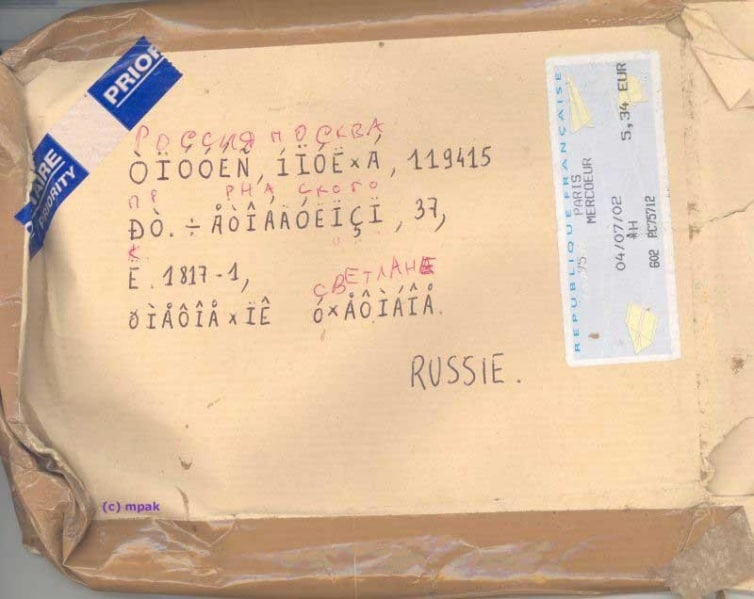
\includegraphics[width=0.8\textwidth]{images/encoding-in-letter.jpg}
  \caption{Справжній лист з плутаниною у кодуванні, який все ж таки був доставлений адресату.}
  \label{PicWrongEncoding}
\end{figure}
}

У будь якому разі, ідея універсального кодування виглядає дуже привабливо.
До цього питання підходили по різному.
Розробники у Microsoft вирішили, що раз одного байту недостатньо, то двох байт точно вистачить всім.
Тому усі нові програми треба було писати у цьому новому кодуванні, це символи складалися з двох байтів.
Старі програми працювали з зоопарком кодувань, як і раніше.
При бажані, розробники могли їх адаптувати так, щоб використовувати двобайтове кодування.
За задумом, у світі мало з'являтися все більше правильних програм, доки неправильні застаріли не стануть атавізмом.

Хотіли як краще, а вийшло як завжди.
По-перше, серед розробників процесорів немає згоди щодо того, який байт треба ставити першим, а який другим.
Це дає два варіанти кодування, про які треба турбуватися.
Трохи детальніше ми обговоримо це у наступному параграфі, але відмітимо, що ці кодування стали позначати \encoding{utf16le} та \encoding{utf16be}.
По-друге, двох байт не вистачило.

\begin{exercise}
На початку параграфу була приведена кількість кодів у стандарті Unicode.
Порахуйте, скільки символів, станом на сьогодні, не влазять у два байти.
\end{exercise}

Інший розв'язок проблеми придумали Кен Томпсон та Роб Пайк.
Головна ідея полягала у тому, щоб кількість байт на символ не була фіксована.
Таким чином, ASCII символи кодувалися би одним байтом, деякі інші символи---двома, більш екзотичні---трьома~і~т.~д.
Так питання сумісності було вирішено: усі старі програми не зламалися, бо для них це нібито окреме кодування, яке отримало назву \encoding{utf8}.\index{кодування, utf8}
До ідеї не фіксованої кількості байт на символ дійшли згодом й у Microsoft.
Символи, які не влізли у два, кодуються чотирма байтами.

Що ж, спробуємо встати на місце Томсона та Пайка, та знову винайдемо кодування \encoding{utf8}.

\begin{exercise}
Спробуйте відкласти книжку та трохи подумати про те, як саме можна закодувати Unicode символи, зі збереженням ASCII кодів символів.
\end{exercise}

Тепер спробуємо зробити якесь пілотне просте рішення, та спробуємо проаналізувати його недоліки.

Добре, що ламати не можна?
Звісно, це коди від \hexstr{00} до \hexstr{7F} включно, бо вони зарезервовані ASCII.
Ці символи не можуть бути навіть частиною багатобайтового символу, бо старі програми будуть їх сприймати як окремі символи.
Тому усі багатобайтні символи маюсь складатися з символів, які мають коди від \hexstr{80} до \hexstr{FF}.
Або, якщо дивитися у двійковій системі числення, старший біт має бути встановлений у одиницю.
Ми будемо писати \bitstr{1ddd~dddd} для того, що показати, що старший біт дорівнює одиниці, а інші біті, яки ми позначити \bitstr{d}, містять дані.

Перша ідея, яка спадає на думку, це додати у перший байт інформацію про кількість байт, які складають один символ.
Якщо виділити на це два біти, то перший байт буде мати вигляд \bitstr{1nnd~dddd}.
Два біти це чотири варіанти, мінімальна кількість байтів це $2$, ще можна задати $3$, $4$ та $5$.
Таким чином, при цьому кодуванні символи не можуть складатися більше ніж зі п'яти символів.

Двобайтні символи будуть складатися з першого байту \bitstr{1nnd~dddd} та другого \bitstr{1ddd~dddd}.
Якщо порахувати кількість бітів, які містять код символу, вони у нас позначені як \bitstr{d}, то ми отримаємо $5+7=12$ біт.
Дванадцять біт, як ми знаємо, це $2^{12}=4096$ варіантів, тобто символи з двох байт можуть закодувати $4096$ різних символів.
Трьохбайтові символи це перший байт \bitstr{1nnd~dddd} за яким ще два \bitstr{1ddd~dddd} та \bitstr{1ddd~dddd}.
Це $5+7+7=19$ біт.
А це майже $2^{19} \approx 500~000$ символів.

\begin{exercise}
Скільки символів можуть містити п'ятибайтові символи?
\end{exercise}

\begin{exercise}
А якщо виділити під довжину символу лише один біт \bitstr{1ndd~dddd}, то скільки символів можна закодувати цим кодуванням?
\end{exercise}

Рішення знайдено? Ні, не усе так просто.
Припустимо, що у нас є результати логування у величезному файлі у сотні гігабайт.
Нам треба знайти у ньому певні цікаві події.
Припустимо, що для прискорення пошук, запустили у двох процесах, один має здійснити пошук у першій половині файлу, а інший у другій.
З першим процесом ніяких проблем немає.
Але з другим...
Припустимо, що він попав на символ з кодом \hexstr{BC}.
Як зрозуміти, це перший байт символу, другий чи третій?
Теоретично може виникнути ситуація, коли ми заплутаємо в байтах, та не зможемо десь поруч знайти початок символу.

Звісно, що це більше \textit{теоретично}.
На практиці у нас десь поруч будуть прогалики \chr{\s}, переноси рядків \chesc n, тому якось викрутитися ми зможемо.
Але на душі неспокійно.
В Unicode є свої еквіваленти для прогаликів, наприклад, той же \boxed{\texttt{NBSP}}.
Також так є різні екзотичні варіанти переносу рядка.
Тому, може особисто в нас ніякої проблеми не буде.
Але ми робимо рішення для всіх, тому можливо що хтось у світі й наступить на граблі.
Тим більше, що рішення цієї проблеми досить просте: треба просто відрізняти перший байт символу від наступних.

Добре, робимо ще один крок у напрямку \encoding{utf8}.
Нехай перший байт буде починатися з \bitstr{11dd~dddd}, а другі, треті, четверті, п'яті, одним словом, не перші, будуть починатися з \bitstr{10dd~dddd}.
Таким чином ми вирішуємо проблему пошуку з середини файлу: щоб синхронізуватися, нам треба піти уперед чи назад або до ASCII символу з кодом \bitstr{0ddd~dddd}, або до першого байту \bitstr{11dd~dddd}.
Ще ми можемо досить легко рухатися по символам у рядку не лише уперед, а й назад.

\begin{exercise}
Опишіть, яким чином ми можемо знайти усі символи у рядку, рухаючись від останнього до першого.
\end{exercise}

Нам лишився останній крок: закодувати довжину у першому байті.
Так, ми можемо виділити на це два біта: \bitstr{11nn~dddd}.
Але тоді двобайтовий символ буде кодувати лише $4+6=10$ біт, $1024$ символи.
Чим менше код символу, тим він частіше зустрічається.
Чи можна якось збільшити діапазон саме для двобайтових символів?
Можна знову знову поділити всі символи на двобайтові та більше ніж двобайтові.
Перші будуть починатися з \bitstr{110d~dddd}, а інші з \bitstr{111d~dddd}.
Таким чином, двобайтовий символ буде складатися з $5+6=11$ біт, а це $2048$ символів.
Виграш у два рази!

Можна продовжити, й поділити решту на трьохбайтові та більше ніж трьохбайтові: \bitstr{1110~dddd} та \bitstr{1111~dddd}.
Трьохбайтові будуть складатися з $4+6+6=16$ біт (два байти), а це $65535$ символів.
Але ми знаємо, що 16 біт не вистачає, тому мають бути ще й чотирьохбайтові, які теж можна поділити на всяк випадок на \bitstr{1111~0ddd} та \bitstr{1111~1ddd}.
Символ з чотирьох байт це $3+6+6+6=21$ біт, або приблизно два мільйони.
Поки що цього вистачає для всіх символів з Unicode.
Але, якщо життя піднесе несподіванку, у нас є решта, яку можна поділити на п'ятибайтові та ще довші.

\begin{exercise}
Якщо продовжувати ділити до переможного кінця, то яка максимальна довжина багатобайтового символу може бути в utf8?
Скільки біт та символів він зможе містити?
\end{exercise}

Поздоровляю, ми ще раз винайшли utf8!

\medskip

Припускаю, що частину читачів поздоровляти зарано.
Дехто продерся через ці пояснення, виключно на морально-вольових якостях, з відчуттям повного нерозуміння справи.
Не хвилюйтесь, це дуже часте явище після читання документації.
Ти або мало розумієш, про що йде мова, або ще гірше---розумієш хибно.
Що ж робити? Експериментувати!
Тільки практика допоможе з'ясувати, як обстоїть діло насправді.

Для експерименту візьмемо тестовий текстовий файл, який складається лише з одного рядка:
\textseq{\texttt{Сік: ₴15}}
\noindent У цьому файлі будуть $14$ байт, у $16$--річній системі числення це будуть наступні байти:
\textseq{\texttt{d0 a1 d1 96 d0 ba 3a 20 e2 82 b4 31 35 0a}}
\noindent Спробуємо розшифрувати цю магію!

Перший байт має код \hexstr{d0}.
Щоб перевести цей код до двійкової системи числення, можна скористатися таблицею~\ref{TableTwoNum}, та отримати \bitstr{1101~0000}.
Проаналізуємо цей байт.
Самий лівий біт встановлено в одиницю, тому це багатобайтний символ.
Він не починається з \bitstr{10}, тому це перший байт символу, що доволі логічно.
Він починається з \bitstr{110}, що означає, що у нас символ складається з двох байт.
Наступні п'ять біт \bitstr{10000} це дані символу, які ми позначимо $h$ та запам'ятаємо.

Другий байт у файлі має код \hexstr{a1}, або \bitstr{1010~0001}.
Самий лівий біт встановлено в одиницю, тому це багатобайтний символ.
Він починається з \bitstr{10}, тобто це не перший байт символу.
Поки що все сходиться, перший байт сказав, що це двобайтовий символ, другий байт це підтвердив.
Наступні шість біт \bitstr{100001} це дані, які ми позначимо $l$ та знову запам'ятаємо.

Тепер у нас є символ, який складається з двох частин $h$ та $l$.
Об'єднуємо їх: $hl = \hbox{\bitstr{10000 100001}}$.
Біти встановлені у позиціях $0$, $5$ та $10$.
Відповідно до формули~\ref{FormulaTwoNum} ми отримаємо Unicode код символу
\begin{equation}
2^{10} + 2^5 + 2^0 = 1024 + 32 + 1 = 1057
\end{equation}
Пошук символу за його кодом дає відповідь, що це велика кирилична літера «С».
Пазл зійшовся.

Але переводити до десятинної системи числення трохи напружує.
Так, ми повторили вивчене раніше, але все ж таки спробуємо з наступним символом дещо інший шлях.
Третій та четвертий байти нашого файлу це \hexstr{d1} та \hexstr{96}, або \bitstr{1101~0001} та \bitstr{1001~0110}.
Знову \hexstr{d1} починається з \bitstr{110}, тобто це перший байт двобайтового символу, дані \bitstr{10001}.
Байт \hexstr{96} починається з \bitstr{10}, тобто це не перший байт, дані \bitstr{010110}.
Поєднуємо дані: \bitstr{10001~010110}.
Раніше ми переводили їх до десятинної системи, зараз просто перегрупуємо по чотири біта \bitstr{100~0101~0110}, та переведемо до $16$--річної системи числення: \hexstr{456}.
Тепер ми маємо $16$--річний Unicode код, який позначається \unicode{0456}.
Пошук у Google виводить нас на сторінку, де можна дізнатися, що символ \unicode{0456} це білоруська-українська маленька літера «і».
Бінго!

\begin{exercise}
П'ятий та шостий байти це \hexstr{d0} та \hexstr{ba}.
Спробуйте знайти десятинний та $16$--річний коди цього символу та знайти його опис.
\end{exercise}

Далі символ з кодом \hexstr{3a}, це ASCII символ, який можна просто підгледіти в таблиці~\ref{TableASCII}, це двокрапка.
Наступний символ \hexstr{20}, це знову ASCII символ, який буде вам зустрічатися доволі часто, бо це прогалик \chr{\s}.
А ось далі цікавіше, нас чекає послідовність \hexstr{e2}, \hexstr{82} та \hexstr{b4}.
Як нескладно здогадатися, це трьохбайтовий символ, але переконаємося у цьому.
Байт \hexstr{e2} це \bitstr{1110~0010}, він починається з \bitstr{1110}, тобто це дійсно трьохбайтовий символ з даними \bitstr{0010}.
Далі йдуть байти \hexstr{82} та \hexstr{b4}, або \bitstr{1000~0010} та \bitstr{1011~0100}, які обидва очікувано починаються з \bitstr{10} (не перші байти).
Дані будуть відповідно \bitstr{000010} та \bitstr{110100}.
Поєднуємо: \bitstr{0010~000010~110100}.
Групуємо по чотири: \bitstr{0010~0000~1011~0100}.
Переводимо у $16$--річний вигляд: «\bitstr{U+20B4}».
Пошук в інтернеті дає відповідь, що цей код відповідає символу валюти української гривні \chr{₴}.

\begin{exercise}
Спробуйте розшифрувати наступні utf8 символи:
\textseq{а) \bitstr{d1 9e}}
\textseq{б) \bitstr{e2 82 a5}}
\textseq{в) \bitstr{f0 9f a4 a3}}
\end{exercise}

\begin{exercise}
А тепер, навпаки, спробуйте побудувати \encoding{utf8} послідовності для символів «\bitstr{U+00A3}», «\bitstr{U+2200}» та «\bitstr{U+1F525}».
\end{exercise}

Сподіваюся, що стало зрозуміліше.
Тому настав час для вправи:

\begin{exercise}
Знову перечитайте опис того, як працює кодування \encoding{utf8} вже з багажем експериментів.
\end{exercise}

Взагалі цикл читання документації, експерименти, повернення до документації, нові експерименти то часта річ у роботі розробника.
Сподіваюся, що ви отримали хоча б маленький досвіт цього протягом читання цього параграфу.

\medskip

Лишилося додати ще пару рис.
Що буде, якщо в нашому файлі поміняти місцями перші два байти, тобто він буде починатися з \bitstr{a1~d0}?
А нічого гарного, бо вже перший символ буде стверджувати, що він не перший.
А де тоді перший?
У кодуванні utf8 не будь яка послідовність байт може бути перетворена у послідовність кодів.
Коли інформація у байтах суперечить одне одній, то ми отримаємо помилку розкодування.
Наприклад, частіше усього це може бути коли ми спробуємо прочитати текст у кодуванні cp866 як utf8.
Як на мене, то краще помилка, ніж вивести кракозяблики та сказати, що та й має бути.

Знову повернемося трохи до Microsoft з її двобайтовими кодуваннями \encoding{utf16le} та \encoding{utf16be}.
Будь який файл може бути або в одному з цих кодувань, або в \encoding{utf8}.
Як можна з'ясувати, яке саме? Ніяк.
Тому було запропоноване рішення починати файл зі службового символу \unicode{FEFF}, який означає прогалик нульової ширини.
Також цей символ отримав назву маркер кодування, BOM (Byte Order Mark).\index{BOM, byte order mark}.
Якщо файл починається зі \bitstr{fe~ff}, то це utf16-be.
Якщо файл починається зі \bitstr{ff~fe}, то це utf16-le.
А якщо файл починається за \bitstr{ef bb bf}, то це utf8.
А якщо файл не починається з цього BOM?
Ну... тоді скоріше за усе це utf8, бо у світі Unix не завжди використовують цей BOM.
Але життя бентежне... трапляється усяке...

\begin{exercise}
Переконайтеся у том, що послідовність байтів \bitstr{ef bb bf} відповідає символу \unicode{FEFF}.
\end{exercise}

\begin{summary}
\item Бажано з повагою ставитися до проблем сумісності та не впровадити рішень, які ламають вже написані програми.
\item Пілотні рішення можуть вас підштовхнути у вірному напрямку.
\item Кодування \encoding{utf8} вирішує проблему обмеженого набору символів, та нічого не ламає.
\item Пам'ятайте цикл документація---експеримент---документація---...
\end{summary}

\section{Числа з байтів}

Ми розпочинали цей розділ з чисел, ми й закінчимо її на числах.
Але, тепер ми знаємо, що процесори зазвичай працюють не з окремими бітами, а з байтами.
Тому трохи обговоримо, як це впливає на числа.
Також ми робили трохи ідеальне припущення, що майже завжди можна вибрати кількість бітів для зберігання значень, яких буде вистачати для усіх можливих варіантів.
Але світ не ідеальний, кількість бітів обирає людина, інколи цей вибір хибний, або також треба на забувати ситуацію, коли дані приходять від зловмисників.
Тому ми також розглянемо, що трапляється в цих випадках.
Також трохи поговоримо про від'ємні числа.

\subsection{Big Engian та Little Endian}

Добре, числа складаються с байтів.
Що це змінює?
Ну, по-перше, кількість біт має бути кратно восьми: якщо число складається з одного байту, то це $8$ біт, якщо з двох байтів, то $16$ біт, і.~т.~п.
По-друге, нам треба домовитися, в якій послідовності будуть розташовані байти.
Розглянемо, наприклад, число, яке складається з двох байт.
Один з байтів буде зберігати перші вісім біт, інший байт останні вісім біт.
Але спочатку має йти байт з першими бітами, чи з останніми?
Наприклад, розглянемо число \hexstr{1122}.
Це 16--бітне число, яке складається з двох байт: \hexstr{11} та \hexstr{22}.
Наше питання полягає у тому, в якому порядку ці байти мають бути розташовані у пам'яті: \bitstr{11~22} чи \bitstr{22~11}?

Це питання здається нам дрібницею, хочеться відразу відреагувати «а яка різниця»?
А різниця відбувається, коди бінарна послідовність байт передається між різними архітектурами комп'ютерів.
А, оскільки, світ не дійшов до згоди у цій «дрібниці», то розробникам інколи треба пам'ятати про різні можливості.

Що ж, спробуємо знайти аргументи за та проти для кожного з них, якими керувалися розробники процесорів.

\begin{exercise}
Спробуйте вибрати один з варіантів, який здається вам більш логічним та правильним.
\end{exercise}

Якщо подивитися на $16$--річний запис числа \hexstr{1122}, то, звичайно, раціональним здається варіант \bitstr{11~22}.
Дійсно, навіщо нам треба заморочуватися та переставляти байти?
Цей спосіб кодування цілих чисел отримав назву Big Engian, та використовується, наприклад, у процесорах ARM.\index{Big Endian}
Думаю, що розв'язуючи попередню вправу більшість читачів обрали саме його.

Зворотній спосіб кодування отримав назву Little Endian, та використовується у процесорах Intell.\index{Little Endian}
Щоб пояснити його обґрунтування, пригадаємо формулу~\ref{FormulaTwoNum} та нумерацію біт, та подивимося пильніше на наше число \hexstr{1122}.
Ми бачимо, що біти з нульового по сьомий складають байт \hexstr{22}, а біти з восьмого по п'ятнадцятий---байт \hexstr{11}.
Тобто байт \hexstr{22} буде містити \textit{перші} біти, а байт \hexstr{11} буде містити \textit{останні} біти.
Тепер варіант \bitstr{11~22} вже не знається нам дуже логічним, бо першими йдуть останні біти, а останніми йдуть перші біти.

\begin{exercise}
Якій послідовності байт у Big Endian та Little Endian буде відповідати число \hexstr{FEFF}, код символу BOF, при який ми говорили наприкінці минулого параграфу?
\end{exercise}

Сподіваюся, що я вас не дуже заплутав цими різними Endian-ами.
Але це граблі, на які інколи наступають й сучасні програмісти, особливо ті, що передають повідомлення з байт, між різними комп'ютерами.

\subsection{Переповнення}

Тепер поговоримо трохи про те, що трапляється коли біт не вистачає для зберігання результату операції.
Наприклад, розробник видів чотири байти для значення зарплатні співробітника.
Це $32$ біти, чого достатньо, бо це трохи більше ніж чотири мільярди.
Достатньо, доки програму не почнуть використовувати у сонячному Зімбабве.

Спробуємо розглянути практичний приклад.
Припустимо у нас є байти $100$ та $200$.
Ми хочемо обчислити їх суму, та записати її у байт.
Але сума буде $300$, а максимальне значення, яке може зберігати байт, це $255$.
Що має відбуватися у цьому випадку?

Ця ситуація отримала назву переповнення.\index{Переповнення}.
Якщо ми беремо банківські транзакції, то, напевне, краще буде у разі переповнення не проводити нічого, повідомити про помилку, та перекласти усю роботу на програмістів, які не подумали про такий випадок.
Але, якщо мова йде про комп'ютерні ігри, то більшість гравців віддасть перевагу, щоб гра проглючила, але продовжувалася.
Тому для розробників процесорів великого вибору немає---треба придумати, як команда має виконуватися найбільш корисним чином, а вже розробники банківських програм мають думати, як зробити так, щоб сумнівні транзакції не проводилися.

Щоб легше було розглядати проблему переповнення, будемо тимчасово вважати, що байт складається с чотирьох біт, бо так їх легко тримати під контролем.
Чотири біта це від $0$ до $15$, або від \bitstr{0} до \bitstr{F}.
Скільки буде $10 + 9$? або \bitstr{1010} + \bitstr{1001} у двійковій системі числення?

Одна з ідей, яка спадає на думку, це узяти максимально можливе значення, у нашому прикладі це $15$.
Обґрунтування досить просте, раз точний результат отримати неможливо, то повернемо максимально близьке значення до нього.
Так, в деяких випадках така поведінка має сенс.
Але, припустимо, що наш процесор вміє додавати лише чотирьохбітні числа, а нам вкрай необхідно запрограмувати додавання восьмибітних.
Наприклад, \hexstr{2A} + \hexstr{39}.
Неважко порахувати, що у результаті має бути \hexstr{63}, але як його отримати?
Подивимося, \bitstr{A} + \bitstr{9} = \hexstr{13}.
Три це остання $16$--річна цифра, її записуємо.
Одиниця каже нам, що було переповнення.
Тому, коли ми будемо додавати \bitstr{2} + \bitstr{3} нам треба не забути ще про цю одиницю, щоб отримати \bitstr{6}.
Точнісінько також ми складаємо й звичайні числа у стовпчик.

\begin{exercise}
Складіть у стовпчик \hexstr{2F} та \hexstr{54}.
\end{exercise}

Це призводить до висновку, що $10 + 9 = 3$ та переповнення.
Саме така логіка й реалізована на більшості процесорів.
\bitstr{1010} + \bitstr{1001} = \bitstr{1~0011}.
Але сама ліва одиничка вже не влазить, тому результат просто дорівнює \bitstr{0011}.

\begin{exercise}
Чому дорівнює $100 + 200$, якщо результат буде записуватися в один звичайний восьмібітний байт?
\end{exercise}

\subsection{Від'ємні числа}

Поговоримо трохи про від'ємні числа.
Припустимо, що нам треба зберегти число $-5$, як це зробити?
Знову, перша думка полягає у тому, щоб зберігати окремо зберігати знак числа, а окремо само число.
Оскільки знак може бути або «$+$», або «$-$», то для зберігання знаку вистачить одного біта.
А якщо відвести під знак старший біт, та домовитися, що \bitstr{0} означатиме «$+$», а \bitstr{1} означатиме «$-$», то усі додатні числа будуть мати однаковий вигляд.

Наприклад, \bitstr{0011}, або \bitstr{0~011}.
Тут \bitstr{0} означає «$+$», \bitstr{011} це $3$, тому \bitstr{0011} це $+3$.
А ось \bitstr{1011} це \bitstr{1~011}.
Тут \bitstr{1} означає «$-$», \bitstr{011} знову $3$, тому \bitstr{1011} це $-3$.

З першого погляду здається, що це непогана ідея.
Це кодування від'ємних чисел отримало назву прямого кодування.\index{від'ємні числа, прямий код}
Дійсно, які можуть бути тут недоліки?
Але є заковика, як інтерпретувати код \bitstr{1~000}.
Ніби то це нуль, але не простий, а зі знаком: «$-0$».
Подібні числа насправді існують, але головна проблема все ж таки полягає у тому, що треба постійно слідкувати, які числа ми додаємо.
Наприклад, \bitstr{0001} + \bitstr{1001}.
Якщо це додатні числа, то $1 + 9 = 10$, або \bitstr{1010}.
Але якщо це від'ємні числа, то $1 + (-1) = 0$, або \bitstr{0000}.
А що робити, коли до додатного числа треба додати від'ємне?

Тому виникає спокуса знайти таке кодування, щоб операції додавання та віднімання виконувалися однаково.
В принципі, таке кодування існує, та його не важко знайти самостійно.
Почнемо з числа $-1$, та придумаємо з ним якусь дію, яка в результаті дасть додатне число, наприклад $(-1) + 1 = 0$.
У двійковій системі числення це буде \bitstr{????} + \bitstr{0001} = \bitstr{0000}.
Якщо уявити, що це додатні числа, то існує єдине число, яке задовольняє цьому рівнянню, це число \bitstr{1111}.
Дійсно, $15 + 1 = 16$, переповнення, та у результаті буде \bitstr{0000}.

Тому усі одиниці це й буде від'ємним числом $-1$.
Далі треба отримати $-2$.
Можна також розглянути $(-2) + 2$, але, для різноманітності, можна розглянути й $(-1) - 1 = -2$.
Число $-1$ ми вже знаємо, це \bitstr{1111}, його додатній аналог це $15$, віднімаємо одиницю, отримуємо $14$ або \bitstr{1110}.

\begin{exercise}
Спробуйте знайти чотирибітну послідовність біт, яка буде відповідати числам $-3$ та $-7$.
\end{exercise}

\afterpage{\begin{longtable}{cccccc}
  \caption{Додатні та від'ємні числа для чисел з чотирьох біт}\\
    Біти & Додатне & Від'ємне & Біти & Додатна & Від'ємне \\ \hline
    \bitstr{0000} & 0 & 0 & \bitstr{1000} &  8 & -8 \\
    \bitstr{0001} & 1 & 1 & \bitstr{1001} &  9 & -7 \\
    \bitstr{0010} & 2 & 2 & \bitstr{1010} & 10 & -6 \\
    \bitstr{0011} & 3 & 3 & \bitstr{1011} & 11 & -5 \\
    \bitstr{0100} & 4 & 4 & \bitstr{1100} & 12 & -4 \\
    \bitstr{0101} & 5 & 5 & \bitstr{1101} & 13 & -3 \\
    \bitstr{0110} & 6 & 6 & \bitstr{1110} & 14 & -2 \\
    \bitstr{0111} & 7 & 7 & \bitstr{1111} & 15 & -1 \\
  \label{TableFourBit}
\end{longtable}}

Ця система кодування отримала назву доповняльний код, та використовується майже усюди.\index{від'ємні числа, доповняльний код}
Щоб було зручно, значення усіх чотирьохбітних послідовностей я навів у таблиці~\ref{TableFourBit} (також буде корисно порівняти цю таблицю, з таблицею~\ref{TableTwoNum}).

\begin{exercise}
Якщо брати байти, то які восьмібітні послідовності будуть відповідати числам $-1$, $-7$ та $-100$?
\end{exercise}

Якщо пильно подивитися на таблицю ~\ref{TableFourBit}, то можна побачити, що чотири біти кодують від'ємні числа від $-8$ до $+7$.
Число $-8$ унікальне в тому плані, що його абсолютне значення (модуль) дорівнює $8$, тобто числу, яке не попадає в діапазон від $-8$ до $+7$.
Тому часто коли описують функцію модуля $\abs x = |x|$, яка працює з цілими числами, то роблять зауваження, що існує одне значення, для якого функція невизначена, або поверне неочікуваний результат.

\begin{exercise}
Який діапазон для від'ємних чисел, які кодуються одним байтом (вісім біт)?
Для якого числа з цієї послідовності неможливо обчислити модуль?
\end{exercise}

\medskip

Вище я писав, що на більшості сучасних процесорів використовується доповняльний код.
Але мова програмування Сі, з якою ми будемо працювати, то вона теж немолода, й виникла ще у ті часи, коли існували різні архітектури процесорів.
Тому у стандарті мови будь які операції, які покладаються на те, що процесор використовує доповнювальний код, вважаються невизначеними.
Якщо дійсно треба бути впевненим у бітовій структурі числа, то треба використовувати додатні числа.
Але на практиці, якщо подивитися що там відбувається у середні, то можна буде побачити доповнювальний код.
В мовах програмування, які з'явилися пізніше, доповнювальний код часто описаний на рівні стандарту, тому розробник може бути впевнений у тому, яка саме послідовність біт відповідатиме від'ємному числу.

\begin{summary}
\item Цілі числа з байтів можливо складати двома різними способами: Big Endian та Little Endian.
\item У разі переповнення, ті біти, яки не «влазять», відкидаються.
\item Від'ємні числа кодуються доповнювальним кодом, процесор може додавати числа не хвилюючись про те, якi саме числа додаються.
\end{summary}


\printindex
\end{document}
